\documentclass[printmode,pl]{mgr}

%opcje klasy dokumentu mgr.cls zostały opisane w dołączonej instrukcji, patrz plik <manual.pdf>

%poniżej deklaracje użycia pakietów, usunąć to co jest niepotrzebne
\usepackage{polski}       %przydatne podczas składania dokumentów w
%j. polskim 
%\usepackage[polish]{babel} %alternatywnie do pakietu
%polski, wybrać jeden z nich
%\usepackage[latin2]{inputenc} %kodowanie znaków, zależne od systemu
%\usepackage[T1]{fontenc} %poprawne składanie polskich czcionek

%pakiety do grafiki
\usepackage{graphicx}
\usepackage{subfigure}
\usepackage{psfrag}

%pakiety dodające dużo dodatkowych poleceń matematycznych
\usepackage{amsmath}
\usepackage{amsfonts}

%pakiety wspomagające i poprawiające składanie tabel
\usepackage{supertabular}
\usepackage{array}
\usepackage{tabularx}
\usepackage{hhline}

%pakiet wypisujący na marginesie etykiety równań i rysunków
%zdefiniowanych przez \label{}, chcąc wygenerować finalną wersję

% \usepackage{showlabels}


\usepackage{microtype}


%definicje własnych poleceń
\newcommand{\R}{I\!\!R} %symbol liczb rzeczywistych, działa tylko w
                        %trybie matematycznym
\newtheorem{theorem}{Twierdzenie}[section] %nowe otoczenie do
                                           %składania twierdzeń

%dane do złożenia strony tytułowej
\title{Aplikacja webowa zwiększająca \\rozdzielczość obrazów}
\engtitle{Master thesis title}
\author{Eryk Wójcik}
\supervisor{dr hab. inż. Andrzej Rusiecki,\\Katedra Informatyki Technicznej}


%\guardian{dr hab. inż. Imię Nazwisko Prof. PWr} %nie używać
%jeśli opiekun jest tą samą osobą co prowadzący pracę

% \date{2023} %standardowo u dołu strony tytułowej umieszczany jest


%poniżej definiuje sie kierunek i ewentualną specjalność
%w obecnej wersji specjalność nie jest wypisywana na stronie tytułowej

\field{Automatyka i Robotyka (AIR)}
\specialisation{ART (ART)}


\usepackage{fontspec}
% \setmainfont{larken}                            % Font family 

\usepackage{hyperref}
\hypersetup{
  colorlinks=true,
  linkcolor=black,
  filecolor=blue,      
  urlcolor=cyan,
}

\usepackage{caption}

\captionsetup[figure]{name=Rys,labelsep=period}     % Zmienia "Rysunek" na "rys" i separator na kropkę
\renewcommand{\thefigure}{\arabic{figure}}          % Usuwa numer sekcji z numeracji rysunku

\setlength{\parindent}{0pt}                         % Usuwa tabulator w paragrafach


\usepackage{pgfplots}
\pgfplotsset{compat=newest}

\begin{document}
\bibliographystyle{plabbrv}

\maketitle
TODO: dodać do bibliografii frameworki i biblioteki użyte w apce
TODO: Comic.png jest z Set14


\tableofcontents

\chapter{Wstęp}



\section{Cel pracy}


Opis celu badań, czyli stworzenia aplikacji webowej służącej do zwiększania rozdzielczości obrazów z użyciem algorytmów ESRGAN i DWSR oraz analiza i porównanie tych algorytmów.



\section{Zakres pracy}


Przedstawienie koncepcji i zagadnień, które zostaną omówione w pracy, w tym wybrane metody i technologie.
% \chapter{Podstawy teoretyczne}

Celem rozdziału jest przedstawienie podstawowych definicji, wytłumaczenie aparatu matematycznego oraz metod wykorzystywanych w algorytmach na których skupia się praca. Dodatkowo ma on na celu ułatwienie dalszego czytania poprzez zapoznanie czytelnika z przyjętymi konwencjami, oznaczeniami oraz symbolami, które mogą pojawić się w kolejnych rozdziałach. 


\section{Definicja super-rozdzielczości}

Super-rozdzielczość (ang. Super-Resolution) odnosi się do procesu poprawy rozdzielczości obrazu lub sekwencji obrazów. W kontekście cyfrowym, super-rozdzielczość jest często realizowana za pomocą algorytmów komputerowych, które mają na celu odtworzenie wysokiej rozdzielczości obrazu [Rys \ref{fig:image2}, \ref{fig:image3}] z jednego lub wielu obrazów o niskiej rozdzielczość [Rys \ref{fig:image1}].

\begin{figure}[ht]
    \centering
    \begin{minipage}[t]{0.3\linewidth}
        
\includegraphics[width=\linewidth]{Rozdziały/02.Podstawy_teoretyczne/Obrazy/comic.png}
        \caption{Obraz oryginalny}
        \label{fig:image1}
    \end{minipage}
    \hspace{0.5cm}
    \begin{minipage}[t]{0.3\linewidth}
        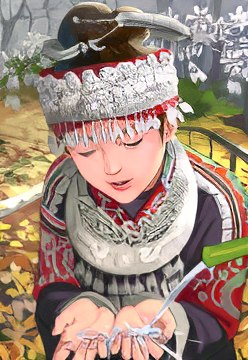
\includegraphics[width=\linewidth]{Rozdziały/02.Podstawy_teoretyczne/Obrazy/comic_ESRGAN_x4.png}
        \caption{Obraz powiększony czterokrotnie}
        \label{fig:image2}
    \end{minipage}
    \hspace{0.5cm}
    \begin{minipage}[t]{0.3\linewidth}
        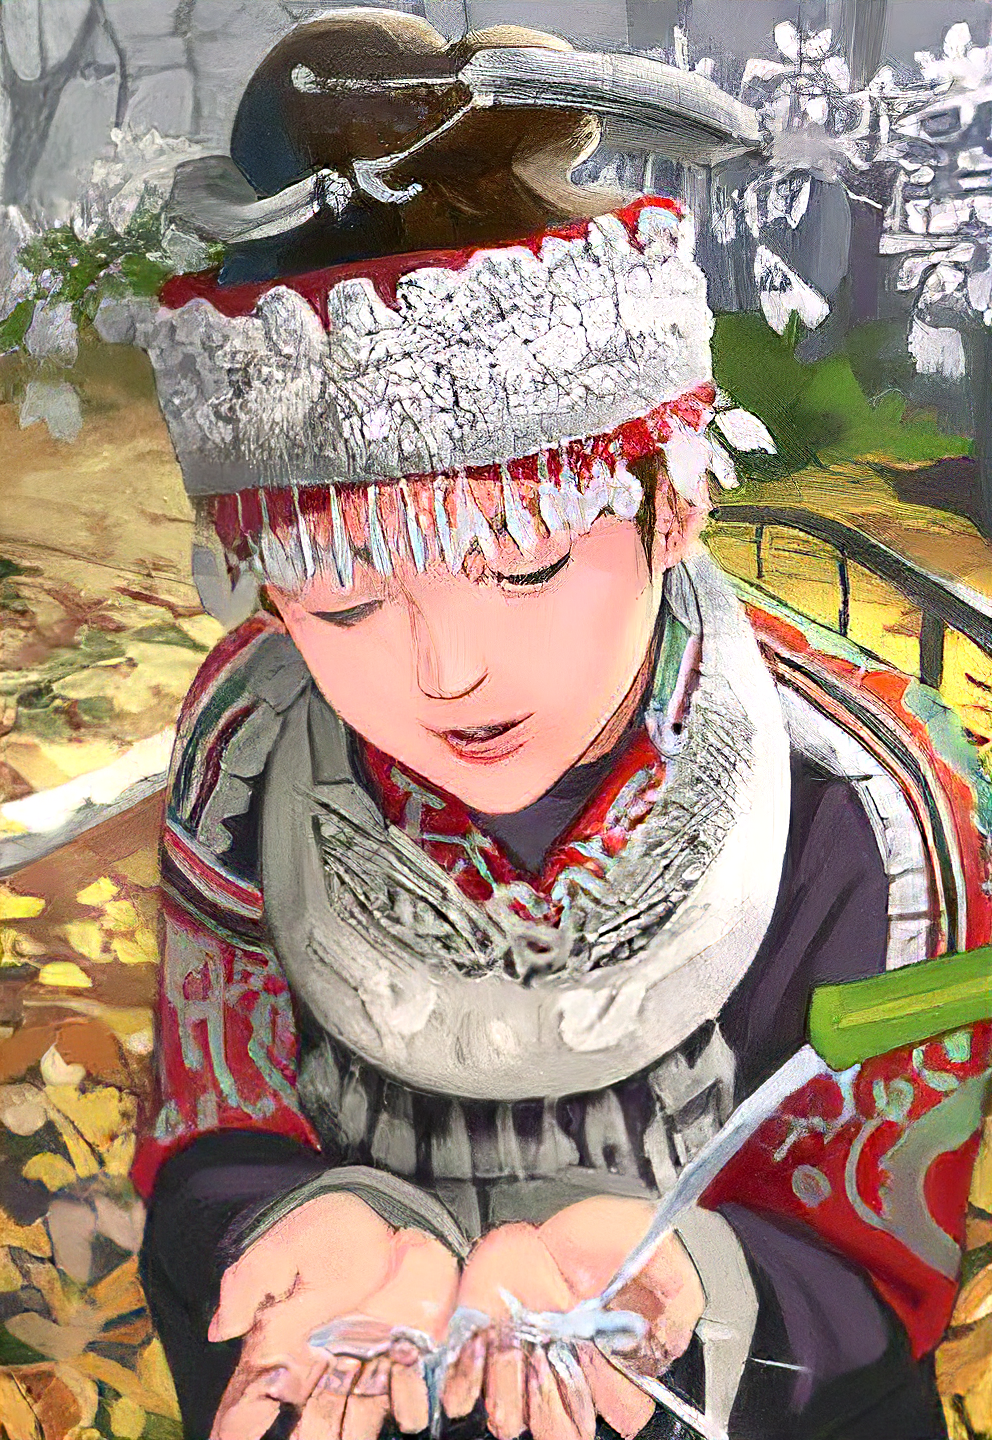
\includegraphics[width=\linewidth]{Rozdziały/02.Podstawy_teoretyczne/Obrazy/comic_ESRGAN_x16.png}
        \caption{Obraz powiększony szesnastokrotnie}
        \label{fig:image3}
    \end{minipage}
\end{figure}

\subsection*{Przykłady zastosowań super-rozdzielczości}

W kontekście praktycznym, techniki super-rozdzielczości znalazły zastosowanie w wielu dziedzinach. Przykładowo, w medycynie, poprawa rozdzielczości obrazów rentgenowskich może znacząco wpływać na dokładność diagnoz. W branży rozrywkowej, technika ta umożliwia remastering starych gier, filmów czy materiałów wideo do standardów HD czy 4K.

W ostatnich miesiącach popularne stało się generowanie obrazów z użyciem sztucznej inteligencji na podstawie podanego opisu tekstowego. Generowane w ten sposób obrazy są określonej wielkości i popularne modele takie jak \textbf{DALL-E} czy \textbf{Midjourney} nie pozwalają na zwiększenie jej. W tym miejscu z pomocą przychodzi super-rozdzielczość, która pozwala na powiększenie obrazu.


\section{Przegląd metod powiększania obrazów}


Istnieje wiele metod powiększania rozdzielczości obrazów. Najprostszą z nich jest \textbf{interpolacja najbliższego sąsiada}, która polega na powieleniu pobliskich pikseli w celu zwiększenia rozdzielczości obrazu. \\
Metoda ta jest bardzo prosta w implementacji, jednakże nie daje ona zadowalających rezultatów. Obraz powiększony w ten sposób wygląda jak obraz o niskiej rozdzielczości z większymi pikselami [Rys \ref{fig:image5}]. 

\begin{figure}[ht]
    \centering
    \begin{minipage}[t]{0.32\linewidth}
        
\includegraphics[width=\linewidth]{Rozdziały/02.Podstawy_teoretyczne/Obrazy/comic.png}
        \caption{Obraz oryginalny}
        \label{fig:image4}
    \end{minipage}
    \hspace{0.5cm}
    \begin{minipage}[t]{0.32\linewidth}
        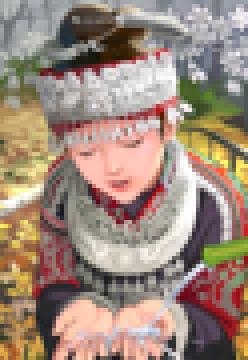
\includegraphics[width=\linewidth]{Rozdziały/02.Podstawy_teoretyczne/Obrazy/comic_NN_x4.png}
        \caption{Obraz powiększony metodą najbliższego sąsiada}
        \label{fig:image5}
    \end{minipage}
  \end{figure}


Aby poprawić jakość obrazu, można zastosować \textbf{interpolację dwuliniową}. Metoda ta rozszerza interpolację liniową na interpolację funkcji dwóch zmiennych [Rys \ref{fig:image6}]. 

\begin{figure}[ht]
    \centering
    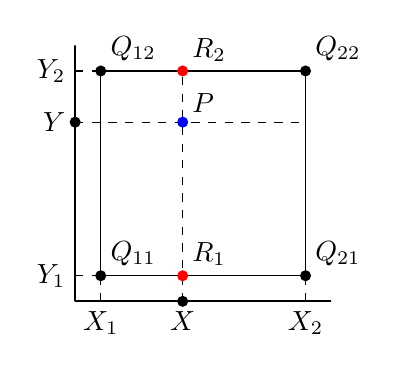
\begin{tikzpicture}[scale=1.3, dot/.style={circle,fill=black,minimum size=4pt,inner sep=0pt,outer sep=-1pt},]

        % Define the coordinates of the grid points
        \coordinate (A) at (1,1);
        \coordinate (B) at (3,1);
        \coordinate (C) at (1,3);
        \coordinate (D) at (3,3);

        \coordinate (R1) at (1.8,1);
        \coordinate (RY) at (1,2.5);
        \coordinate (R1end) at (1.8,3);
        \coordinate (RYend) at (3,2.5);

        \coordinate (P) at (1.8,2.5);

        \coordinate (X) at (1.8,0.75);
        \coordinate (Y) at (0.75,2.5);
        \coordinate (X1) at (1,0.75);
        \coordinate (X2) at (3,0.75);
        \coordinate (Y1) at (0.75,1);
        \coordinate (Y2) at (0.75,3);
        
        \coordinate (frameS) at (0.75,0.75);
        \coordinate (frameX) at (3.25,0.75);
        \coordinate (frameY) at (0.75,3.25);


        \draw[thick] (frameS) rectangle (frameX);
        \draw[thick] (frameS) rectangle (frameY);
        
        \draw[thin] (A) rectangle (D);
        
        % Draw lines from corners to the interpolated point
        \draw[dashed] (X) -- (R1end);
        \draw[dashed] (Y) -- (RYend);
        \draw[dashed] (X1) -- (A);
        \draw[dashed] (X2) -- (B);
        \draw[dashed] (Y1) -- (A);
        \draw[dashed] (Y2) -- (C);

        % Draw the dots
        \node[dot] at (A) {};
        \node[dot] at (B) {};
        \node[dot] at (C) {};
        \node[dot] at (D) {};
        \node[dot, blue] at (P) {};
        \node[dot, red] at (R1) {};
        \node[dot, red] at (R1end) {};
        \node[dot] at (X) {};
        \node[dot] at (Y) {};
        
        % Labels for the corners
        \node[above right] at (A) {$Q_{11}$};
        \node[above right] at (B) {$Q_{21}$};
        \node[above right] at (C) {$Q_{12}$};
        \node[above right] at (D) {$Q_{22}$};
        
        % Label for the interpolated point
        \node[above right] at (P) {$P$};

        \node[above right] at (R1) {$R_{1}$};
        \node[above right] at (R1end) {$R_{2}$};
        \node[below] at (X) {$X$};
        \node[left] at (Y) {$Y$};
        \node[below] at (X1) {$X_{1}$};
        \node[below] at (X2) {$X_{2}$};
        \node[left] at (Y1) {$Y_{1}$};
        \node[left] at (Y2) {$Y_{2}$};
        

        % Add title
        % \node[below] at (current bounding box.south) {Wizualizacja interpolacji dwuliniowej};

    \end{tikzpicture}
    
    \caption{Wizualizacja interpolacji dwuliniowej}
    \label{fig:image6}
\end{figure}


W efekcie polega to na wyznaczeniu średniej ważonej pikseli sąsiadujących z pikselem, który chcemy powielić. Współczynniki wag są wyznaczane na podstawie odległości od piksela, który chcemy powielić.
Kroki algorytmu:
\begin{enumerate}
    \item Przeprowadzana jest interpolacja liniowa wzdłuż osi $O X$:
    
    $$
    \begin{array}{llll}
    f\left(R_1\right) \approx \frac{x_2-x}{x_2-x_1} f\left(Q_{11}\right)+\frac{x-x_1}{x_2-x_1} f\left(Q_{21}\right) & \text { gdzie } & R_1=\left(x, y_1\right), \\ \\
    f\left(R_2\right) \approx \frac{x_2-x}{x_2-x_1} f\left(Q_{12}\right)+\frac{x-x_1}{x_2-x_1} f\left(Q_{22}\right) & \text { gdzie } & R_2=\left(x, y_2\right) .
    \end{array}
    $$
    \item Następnie przeprowadzana jest interpolacja wzdłuż osi $O Y$:
    $$
    f(P) \approx \frac{y_2-y}{y_2-y_1} f\left(R_1\right)+\frac{y-y_1}{y_2-y_1} f\left(R_2\right) .
    $$
\end{enumerate}


W efekcie otrzymujemy obraz wyglądający następująco [Rys \ref{fig:image8},  \ref{fig:image10}].


\begin{figure}[ht]
    \centering
    \begin{minipage}[t]{0.33\linewidth}
        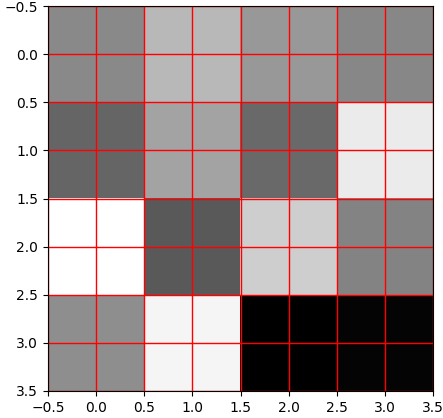
\includegraphics[width=\linewidth]{Rozdziały/02.Podstawy_teoretyczne/Obrazy/bilinear_original.png}
        \caption{Obraz wejściowy}
        \label{fig:image7}
    \end{minipage}
    \hspace{0.5cm}
    \begin{minipage}[t]{0.33\linewidth}
        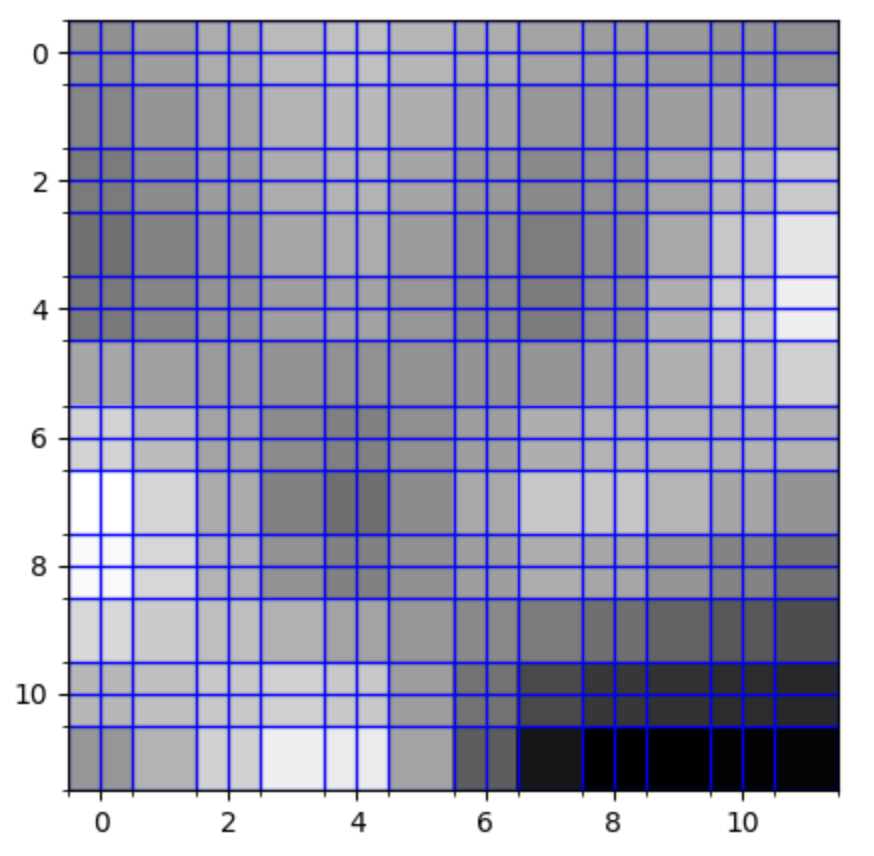
\includegraphics[width=\linewidth]{Rozdziały/02.Podstawy_teoretyczne/Obrazy/bilinear_enlarged.png}
        \caption{Obraz powiększony przez interpolację dwuliniową}
        \label{fig:image8}
    \end{minipage}
\end{figure}

\begin{figure}[ht]
    \centering
    \begin{minipage}[t]{0.33\linewidth}
        
\includegraphics[width=\linewidth]{Rozdziały/02.Podstawy_teoretyczne/Obrazy/comic.png}
        \caption{Obraz wejściowy}
        \label{fig:image9}
    \end{minipage}
    \hspace{0.5cm}
    \begin{minipage}[t]{0.33\linewidth}
        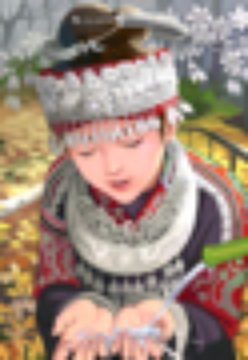
\includegraphics[width=\linewidth]{Rozdziały/02.Podstawy_teoretyczne/Obrazy/comic_BILINEARx4.png}
        \caption{Obraz powiększony przez interpolację dwuliniową}
        \label{fig:image10}
    \end{minipage}
\end{figure}


Metoda ta daje lepsze rezultaty niż interpolacja najbliższego sąsiada, jednakże wprowadziła ona duże rozmycie, które jest szczególnie widoczne na krawędziach obiektów i obszarach wysokiej częstotliwości.

\subsection*{Teoria informacji}

W teorii informacji istnieje koncepcja zwana \textbf{nierównością przetwarzania danych}. Zgodnie z nią niezależnie od sposobu przetwarzania danych, \textbf{nie można dodać informacji, której nie ma w oryginalnej serii danych}  [Wzór 2.1].

\begin{equation}
    \begin{gathered}
    X \rightarrow Y \rightarrow Z \\
    I(X ; Y) \geq I(X ; Z)
    \end{gathered}
\end{equation}

Oznacza to, że brakujących danych nie można odzyskać poprzez dalsze przetwarzanie. Czy to oznacza, że super-rozdzielczość jest teoretycznie niemożliwa? 

Nie, jeśli mamy dodatkowe źródło informacji. 


% \newpage
\section{Wprowadzenie do głębokiego uczenia się w przetwarzaniu obrazów}

Głębokie uczenie rewolucjonizuje przetwarzanie obrazów, wprowadzając modele zdolne do uczenia się cech z serii danych. W przetwarzaniu obrazów, głębokie sieci neuronowe są wykorzystywane do zadań takich jak detekcja obiektów, segmentacja, klasyfikacja obrazów, czy właśnie super-rozdzielczość [Rys \ref{fig:image12},  \ref{fig:image13}].

\begin{figure}[ht]
    \centering
    \begin{minipage}[t]{0.3\linewidth}
        
\includegraphics[width=\linewidth]{Rozdziały/02.Podstawy_teoretyczne/Obrazy/comic.png}
        \caption{Obraz wejściowy}
        \label{fig:image11}
    \end{minipage}
    \hspace{0.5cm}
    \begin{minipage}[t]{0.3\linewidth}
        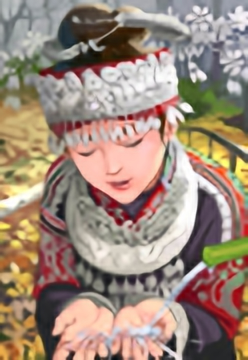
\includegraphics[width=\linewidth]{Rozdziały/02.Podstawy_teoretyczne/Obrazy/comic_DWSR_x4.png}
        \caption{Obraz powiększony algorytmem DWSR}
        \label{fig:image12}
    \end{minipage}
    \hspace{0.5cm}
    \begin{minipage}[t]{0.3\linewidth}
        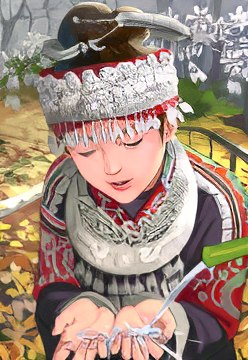
\includegraphics[width=\linewidth]{Rozdziały/02.Podstawy_teoretyczne/Obrazy/comic_ESRGAN_x4.png}
        \caption{Obraz powiększony algorytmem ESRGAN}
        \label{fig:image13}
    \end{minipage}
\end{figure}

Sieć neuronowa może nauczyć się odtwarzać szczegóły obrazów na podstawie pewnych informacji, które zbiera z dużego zbioru obrazów. 

Szczegóły dodawane do powiększanego obrazu w przy użyciu modelu uczenia maszynowego nie naruszają nierówności przetwarzania danych, ponieważ wykorzystywane informacje są w zbiorze treningowym, nawet jeśli nie ma ich na obrazie wejściowym.





\subsection*{Podstawy Głębokiego Uczenia}
Głębokie uczenie, będące zaawansowaną formą uczenia maszynowego, wykorzystuje wielowarstwowe sieci neuronowe do analizy i interpretacji dużych zbiorów danych. Te sieci składają się z warstw skomplikowanych struktur algorytmicznych, które naśladują sposób, w jaki ludzki mózg przetwarza informacje.


\subsubsection*{Architektura Sieci Neuronowych}
Architektura sieci neuronowych w głębokim uczeniu charakteryzuje się wieloma ukrytymi warstwami, które pozwalają na przetwarzanie danych na różnych poziomach abstrakcji. Każda warstwa składa się z wielu neuronów, z których każdy otrzymuje dane wejściowe, przetwarza je i przekazuje dalej. Istnieją różne rodzaje warstw, w tym:
\begin{itemize}
    \item \textbf{Warstwy konwolucyjne (Convolutional Layers)}: Są fundamentem sieci konwolucyjnych (CNNs), które są szeroko stosowane w przetwarzaniu obrazów. Te warstwy stosują filtr konwolucyjny do danych wejściowych, wydobywając lokalne cechy, takie jak krawędzie, kształty czy tekstury.
    \item \textbf{Warstwy pooling (Pooling Layers)}: Redukują wymiarowość danych, jednocześnie zachowując ważne informacje. Najczęściej stosowanymi są max pooling i average pooling.
    \item \textbf{Warstwy w pełni połączone (Fully Connected Layers)}: Każdy neuron w tych warstwach jest połączony ze wszystkimi neuronami w poprzedniej warstwie, co pozwala na integrację nauczonej wiedzy z poprzednich warstw.
\end{itemize}


\subsubsection*{Funkcje Aktywacji}
Funkcje aktywacji w sieciach neuronowych to nieliniowe transformacje stosowane do wyjść neuronów. Pozwalają one na modelowanie złożonych zależności między danymi wejściowymi a wyjściowymi. W głębokim uczeniu stosuje się różne funkcje aktywacji, w tym:
\begin{itemize}
    \item \textbf{ReLU (Rectified Linear Unit)}: Przekształca wszystkie ujemne wartości na zero, podczas gdy wartości dodatnie pozostają niezmienione  [Rys \ref{fig:image14}].
    \item \textbf{Sigmoid}: Przyjmuje wartości wejściowe i konwertuje je na wartości z zakresu od 0 do 1 [Rys \ref{fig:image15}].
    \item \textbf{Tanh (Hyperbolic Tangent)}: Podobnie jak sigmoid, ale konwertuje wartości na zakres od -1 do 1 [Rys \ref{fig:image16}].
\end{itemize}

\begin{figure}[ht]
    \centering
    \begin{minipage}[t]{0.3\linewidth}
        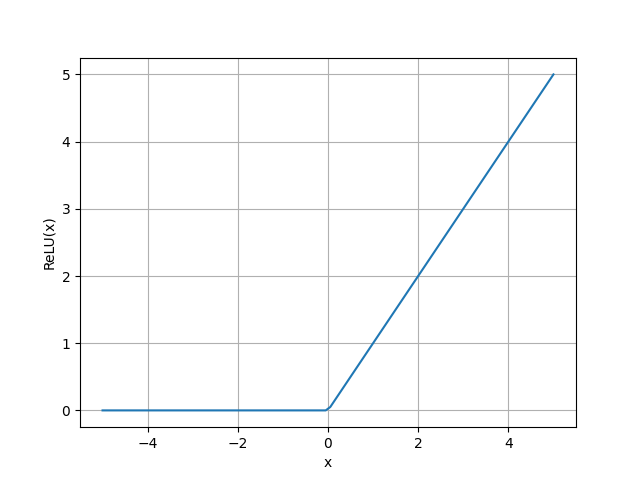
\includegraphics[width=\linewidth]{Rozdziały/02.Podstawy_teoretyczne/Obrazy/relu.png}
        \caption{ReLU}
        \label{fig:image14}
    \end{minipage}
    \hspace{0.5cm}
    \begin{minipage}[t]{0.3\linewidth}
        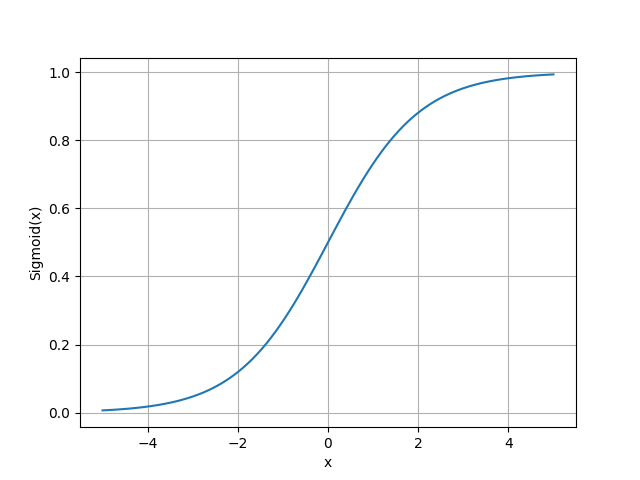
\includegraphics[width=\linewidth]{Rozdziały/02.Podstawy_teoretyczne/Obrazy/sigmoid.png}
        \caption{Sigmoid}
        \label{fig:image15}
    \end{minipage}
    \hspace{0.5cm}
    \begin{minipage}[t]{0.3\linewidth}
        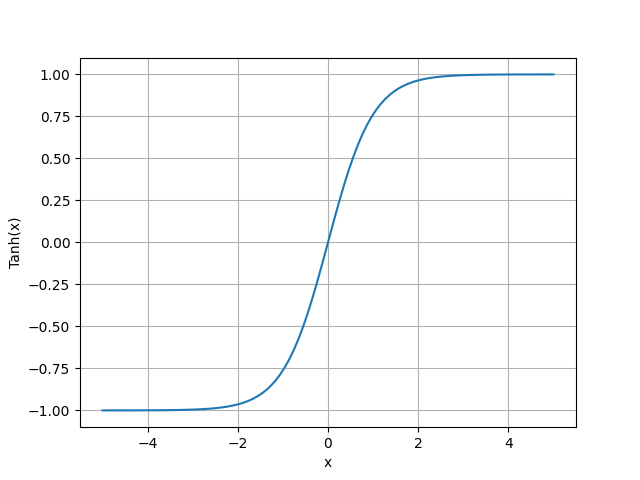
\includegraphics[width=\linewidth]{Rozdziały/02.Podstawy_teoretyczne/Obrazy/tanh.png}
        \caption{Tanh}
        \label{fig:image16}
    \end{minipage}
\end{figure}


\subsubsection*{Strategie Uczenia w Głębokim Uczeniu}
Głębokie uczenie obejmuje różne strategie uczenia, które są stosowane w zależności od rodzaju i charakteru danych oraz oczekiwanych wyników. Do głównych strategii należą:

\begin{itemize}
    \item \textbf{Uczenie nadzorowane (Supervised Learning)}: W tym podejściu model uczy się na podstawie zestawu danych, które zawierają zarówno dane wejściowe, jak i odpowiednie etykiety. Jest to szeroko stosowane w zadaniach takich jak np. klasyfikacja.
    \item \textbf{Uczenie nienadzorowane (Unsupervised Learning)}: Model próbuje znaleźć wzorce w danych bez etykiet, stosowane głównie w grupowaniu i redukcji wymiarowości.
    \item \textbf{Uczenie ze wzmacnianiem (Reinforcement Learning)}: W tej strategii agent uczy się podejmować decyzje poprzez interakcje z otoczeniem, dążąc do maksymalizacji sumy nagród.
\end{itemize}


\subsubsection*{Przeuczenie i Generalizacja}

Przeuczenie (Overfitting) występuje, gdy model zbyt dokładnie dopasowuje się do danych treningowych, tracąc zdolność do efektywnego działania na nowych danych [Rys \ref{fig:image17}]. Niebieska linia reprezentuje przeuczony model, zaś czarna dopasowany. Widać że niebieska linia podąża za danymi treningowymi, jest zbyt zależna od nich co sprawia, że model przeuczony będzie miał wyższy poziom błędu dla nowych danych. Jest to problem szczególnie w przypadku zbyt skomplikowanych modeli w stosunku do danych.
\begin{figure}[h]
    \centering
    
\includegraphics[width=0.4\linewidth]{Rozdziały/02.Podstawy_teoretyczne/Obrazy/overfitting.png}
    \caption{Wizualizacja przeuczenia}
    \label{fig:image17}
\end{figure}

Celem jest stworzenie modelu, który efektywnie działa na nowych, nieznanych danych, co oznacza, że model jest dobrze dostosowany do rzeczywistych scenariuszy.

Przykładowe sposoby na zapobieganie przeuczeniu:

\begin{itemize}
    \item \textbf{Wczesne zatrzymywanie (early stopping):} Polega na monitorowaniu wydajności modelu na zestawie walidacyjnym i zatrzymaniu treningu, gdy wydajność przestaje się poprawiać, co zapobiega przeuczeniu.
    \item \textbf{Walidacja krzyżowa (cross-validation):} Metoda oceny modelu, w której zestaw danych dzieli się na kilka części. Model jest następnie trenowany na jednej części (zwanej zestawem treningowym) i walidowany na innej (zwanej zestawem walidacyjnym), co jest powtarzane na różnych kombinacjach części danych. Pozwala to na lepszą ocenę zdolności modelu do generalizacji na nieznanych danych.s
    \item \textbf{Augmentacja danych (data augmentation):} Zwiększa różnorodność danych treningowych poprzez wprowadzenie niewielkich losowych zmian, co pomaga modelowi lepiej uogólnić i zmniejszyć przeuczenie.
\end{itemize}


\subsection*{Algorytmy Głębokiego Uczenia w Super-Rozdzielczości}

\begin{figure}[h]
    \centering
    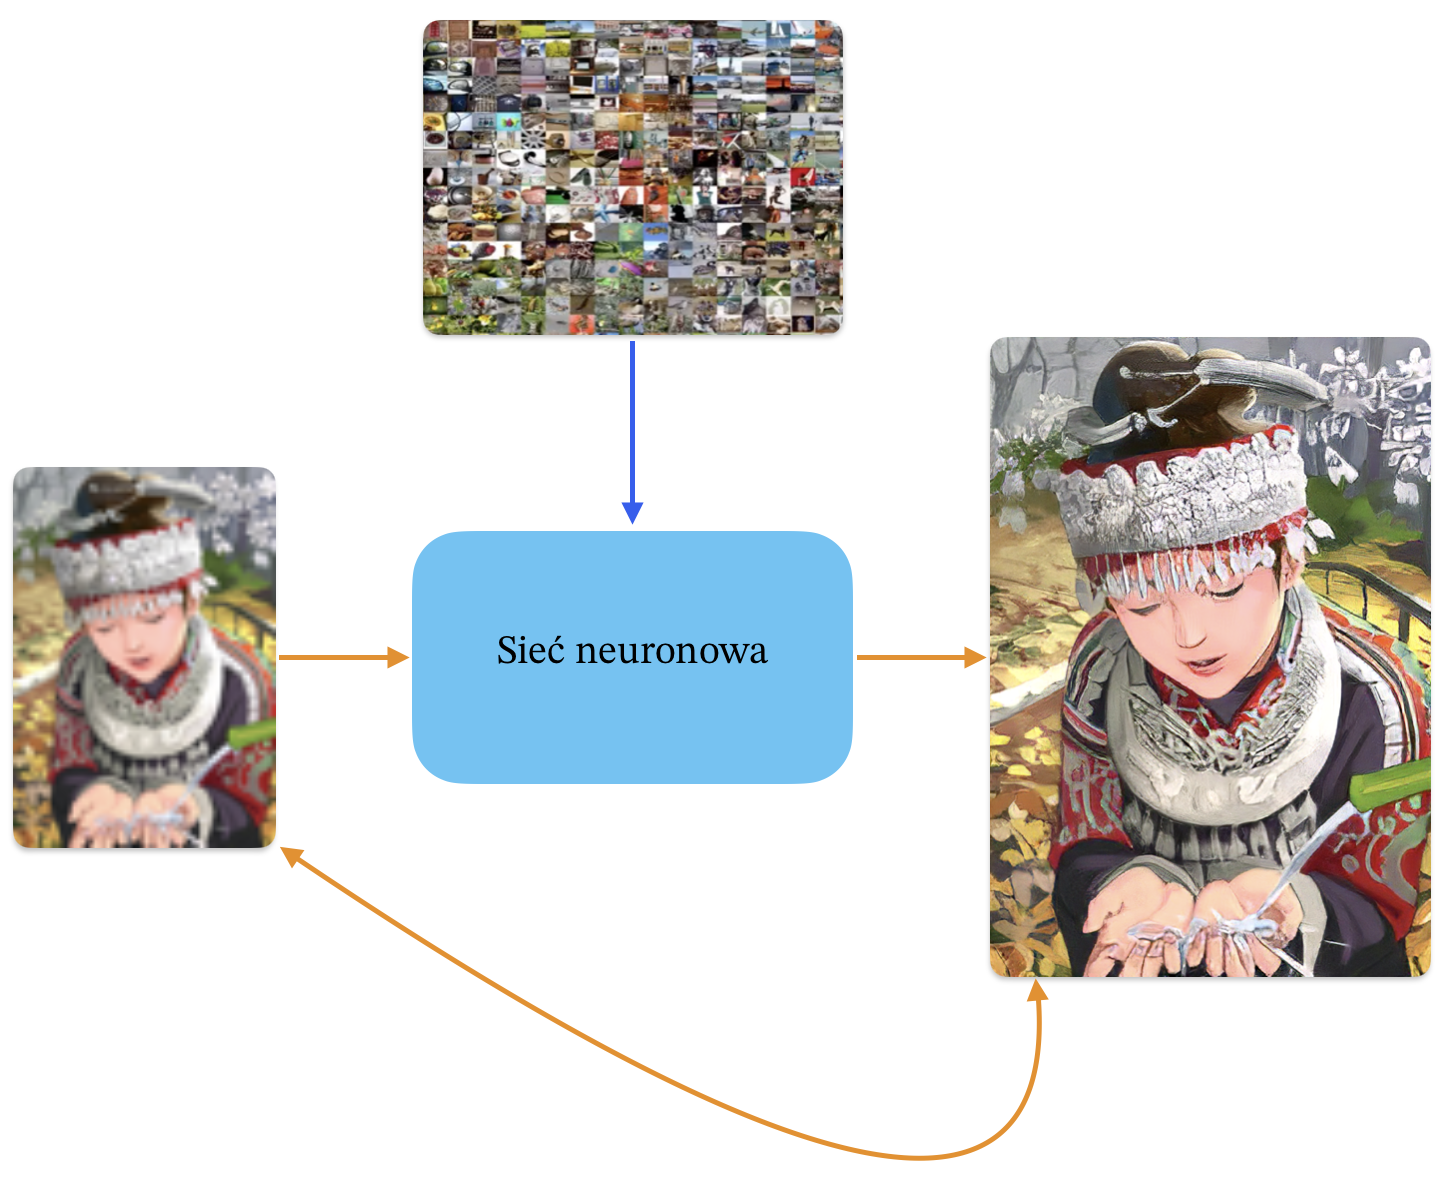
\includegraphics[width=0.5\linewidth]{Rozdziały/02.Podstawy_teoretyczne/Obrazy/map_low-hi_res.png}
    \caption{}
    \label{fig:image18}
\end{figure}



\subsubsection*{Mean Squared Error (MSE)}
\cite{4775883}

W tej pracy opisywane będą szczegółowo dwa bardzo ciekawe algorytmy głębokiego uczenia stosowane w zadaniu super-rozdzielczości. Jeden z nich wykorzystuje 


\newpage
\section{Wstęp do transformacji falkowej}


Transformacja falkowa (wavelet transform) stanowi istotne narzędzie w analizie sygnałów i przetwarzaniu obrazów, zwłaszcza w kontekście zastosowań takich jak super rozdzielczość. Charakterystyczna dla funkcji falkowych jest ich zdolność do dostosowania się do wymagań analizy sygnału. W przeciwieństwie do transformacji Fouriera, która skupia się wyłącznie na częstotliwości, falki pozwalają na efektywną lokalizację zjawisk w sygnale, uwzględniając zmiany zarówno w czasie, jak i częstotliwości.

\begin{figure}[ht]
    \centering

    \begin{minipage}[t]{0.3\linewidth}
        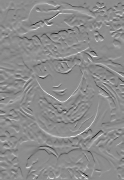
\includegraphics[width=\linewidth]{Rozdziały/02.Podstawy_teoretyczne/Obrazy/horizontal_detail.png}
        \caption{Detale poziome}
        \label{fig:image19}
    \end{minipage}
    \hspace{0.5cm}
    \begin{minipage}[t]{0.3\linewidth}
        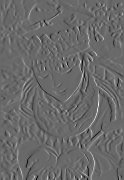
\includegraphics[width=\linewidth]{Rozdziały/02.Podstawy_teoretyczne/Obrazy/vertical_detail.png}
        \caption{Detale pionowe}
        \label{fig:image20}
    \end{minipage}
    \hspace{0.5cm}
    \begin{minipage}[t]{0.3\linewidth}
        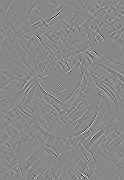
\includegraphics[width=\linewidth]{Rozdziały/02.Podstawy_teoretyczne/Obrazy/diagonal_detail.png}
        \caption{Detale diagonalne}
        \label{fig:image21}
    \end{minipage}
\end{figure}\

W kontekście super rozdzielczości, funkcje falkowe są wykorzystywane do zwiększania jakości obrazów i sygnałów poprzez umożliwienie dokładniejszej analizy i rekonstrukcji ich składowych. Mamy informacje o kierunkach i wielkościach częstotliwości w analizowanym obrazie [Rys \ref{fig:image19}, \ref{fig:image20} \ref{fig:image21}]. 
% Korzystając z funkcji falkowych mamy informacje o kierunkach częstotliwości w analizowanym obrazie, co sprawia że wiemy jak ukierunkowane są krawędzie i tekstury. 
% Dzięki swoim właściwościom, falki potrafią efektywnie oddzielać istotne cechy sygnału od szumu, co jest istotne w procesie zwiększania rozdzielczości.


\subsubsection{Dziedzina czasu i częstotliwości}

Dziedzina czasu odnosi się do analizy sygnału w zakresie czasu, co oznacza, że sygnał jest przedstawiany i analizowany w kontekście jego zmian w czasie. Jest to intuicyjna forma reprezentacji sygnałów, niemniej jednak nie daje ona nam pełnej informacji o sygnale. Z drugiej strony sygnał możemy określić w dziedzinie częstotliwości, która koncentruje się na analizie częstotliwościowych składników sygnału.

% W przetwarzaniu obrazów dziedzina częstotliwości jest często stosowana na przykład do usuwania szumów, wykrywania wzorców i stosowania różnych filtrów.

\begin{figure}[h]
    \centering
    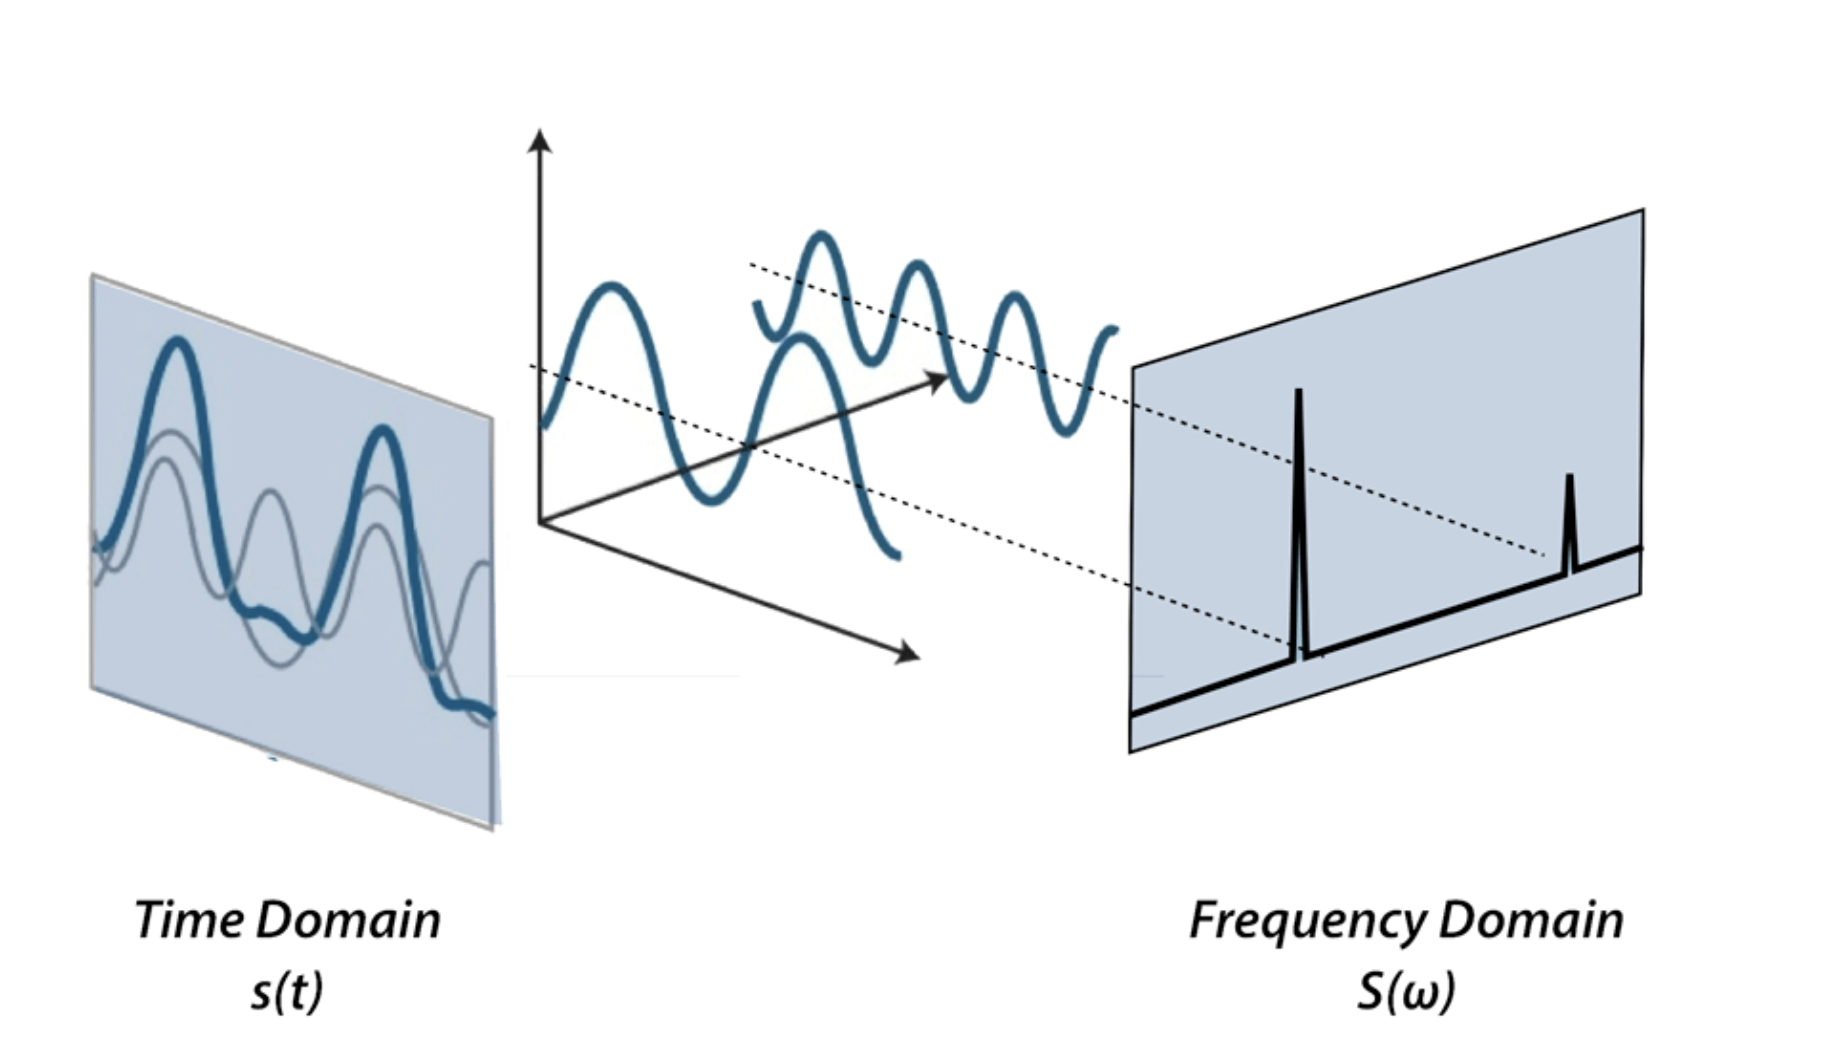
\includegraphics[width=0.47\linewidth]{Rozdziały/02.Podstawy_teoretyczne/Obrazy/time-frequency-domain.png}
    \caption{Wizualizacja dziedziny czasu i częstotliwości}
    \label{fig:image22}
\end{figure}



\subsection*{Transformata Fouriera}

Transformacja Fouriera jest algorytmem używanym do konwersji sygnału z dziedziny czasu do dziedziny częstotliwości. Pozwala ona na uzyskanie widma amplitudowego i fazowego, które prezentują częstotliwości występujące w sygnale i ich amplitudy.

\begin{figure}[h]
    \centering
    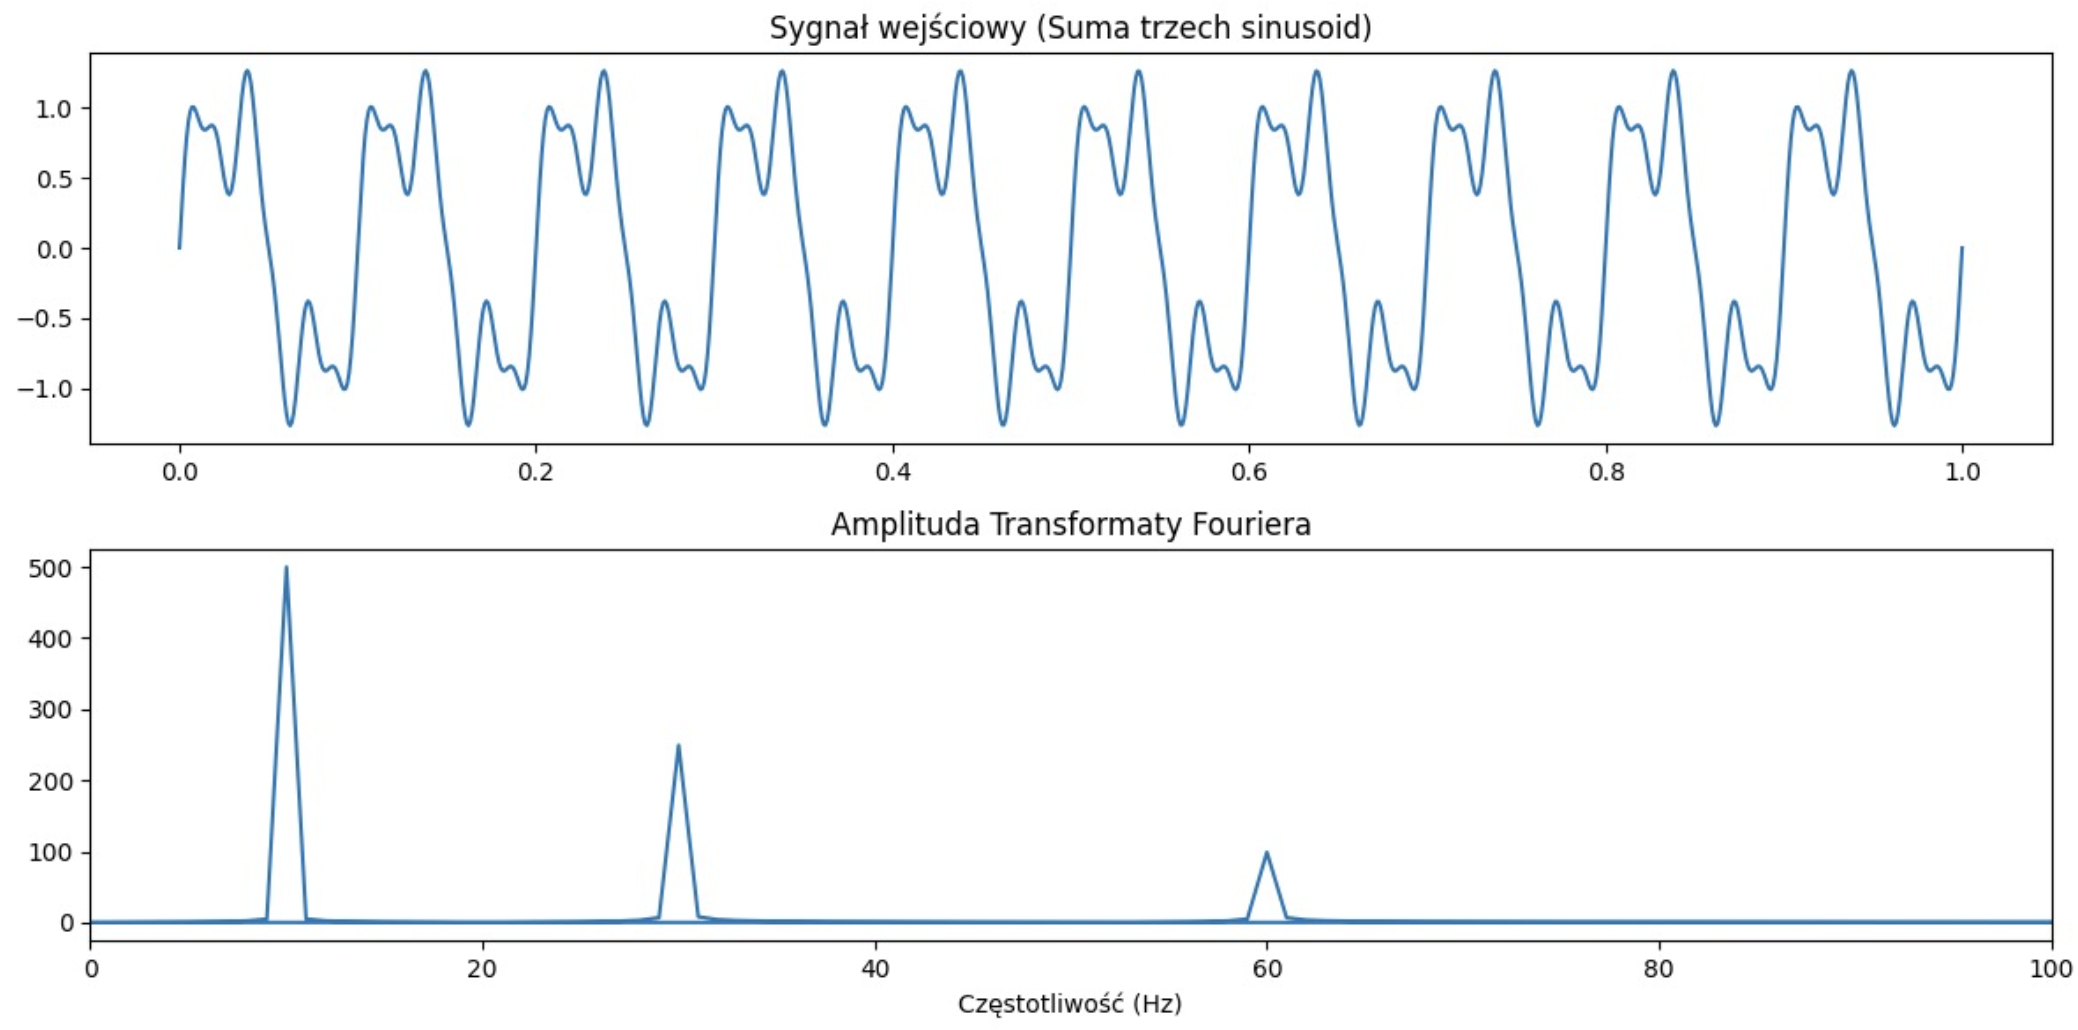
\includegraphics[width=0.8\linewidth]{Rozdziały/02.Podstawy_teoretyczne/Obrazy/fft.png}
    \caption{Wynik transformacji Fouriera dla przykładowego sygnału}
    \label{fig:image23}
\end{figure}

W kontekście przetwarzania obrazów, transformata Fouriera jest stosowana przekształcenia obrazu do dziedziny częstotliwościowej. Wynik transformacji Fouriera jest liczbą zespoloną, która może być reprezentowana jako wektor złożony z dwóch części: rzeczywistej i urojonej, co być przedstawione w postaci dwóch wykresów: amplitudowego i fazowego [Rys \ref{fig:image25}, \ref{fig:image26}].

\begin{figure}[ht]
    \centering
    \begin{minipage}[t]{0.325\linewidth}
        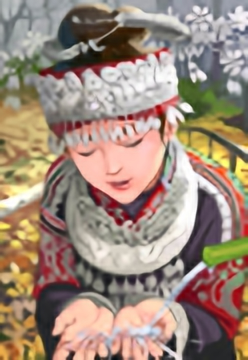
\includegraphics[width=\linewidth]{Rozdziały/02.Podstawy_teoretyczne/Obrazy/comic_DWSR_x4.png}
        \caption{Obraz wejściowy}
        \label{fig:image24}
    \end{minipage}
    % \hspace{0.5cm}
    \begin{minipage}[t]{0.325\linewidth}
        
\includegraphics[width=\linewidth]{Rozdziały/02.Podstawy_teoretyczne/Obrazy/fft_magnitude.png}
        \caption{Wykres amplitudowy}
        \label{fig:image25}
    \end{minipage}
    % \hspace{0.5cm}
    \begin{minipage}[t]{0.325\linewidth}
        
\includegraphics[width=\linewidth]{Rozdziały/02.Podstawy_teoretyczne/Obrazy/fft_phase.png}
        \caption{Wykres fazowy}
        \label{fig:image26}
    \end{minipage}
\end{figure}\

Transformacja Fouriera jest operacją odwracalną, co oznacza, że można ją wykorzystać do rekonstrukcji oryginalnego sygnału z częstotliwościowej reprezentacji stosując odwrotną transformację Fouriera.


\subsubsection{Ograniczenia Transformacji Fouriera}

Zgodnie z zasadą nieoznaczoności Heisenberga nie można jednocześnie precyzyjnie określić i lokalizować zjawisk zarówno w dziedzinie czasu, jak i częstotliwości, zawsze mamy do czynienia z kompromisem. 
\begin{equation*}
    \Delta f \Delta t \geq 1
\end{equation*}
Możemy albo dokładnie określić wartość sygnału w czasie, albo dokładnie określić jego częstotliwość, ale nie możemy zrobić obu jednocześnie.

W rezultacie, podczas gdy Transformata Fouriera oferuje doskonałą rozdzielczość częstotliwościową, traci na zdolności do lokalizacji zjawisk w czasie. Oznacza to, że badając sygnał wyłącznie w dziedzinie częstotliwości, wiemy jakie częstotliwości występują, ale nie jesteśmy w stanie określić kiedy występuje dana częstotliwość.

Czy istnieje narzędzie pozwalające nam na dokładniejszą analizę sygnału? Kompromis pomiędzy czasem a częstotliwością jest nieunikniony, ale istnieje sposób na poprawę lokalizacji w czasie kosztem rozdzielczości częstotliwościowej? Odpowiedzią na te pytania jest transformacja falkowa.


\subsection*{Funkcje Falkowe}

Gdy wykonujemy transformatę Fouriera rozdzielamy sygnał na sumę sinusoid i cosinusoid o różnych częstotliwościach. Funkcje falkowe są podobne do funkcji sinusoidalnych, ale różnią się od nich tym, że mają skończoną długość i są ograniczone do określonego obszaru [Rys \ref{fig:image27}, \ref{fig:image28}].

\begin{figure}[ht]
    \centering
    \begin{minipage}[t]{0.45\linewidth}
        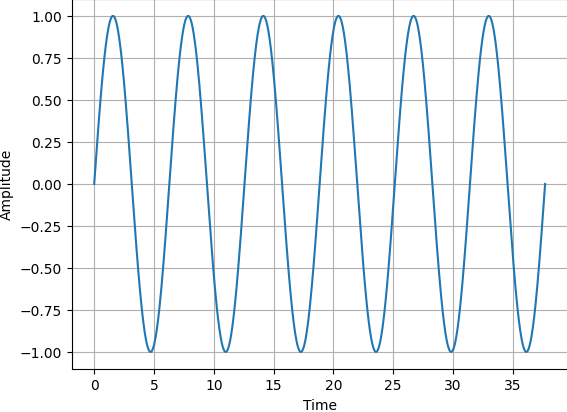
\includegraphics[width=\linewidth]{Rozdziały/02.Podstawy_teoretyczne/Obrazy/sine_wave.png}
        \caption{Sinusoida}
        \label{fig:image27}
    \end{minipage}
    \hspace{0.5cm}
    \begin{minipage}[t]{0.45\linewidth}
        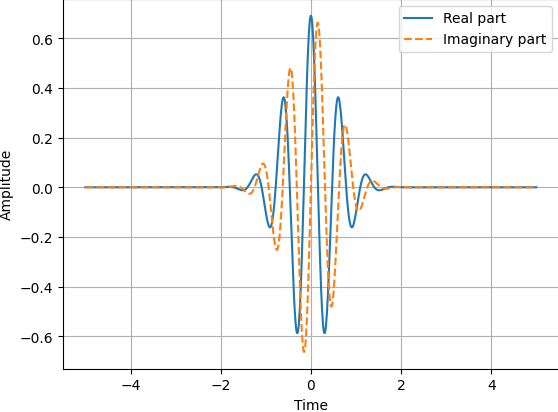
\includegraphics[width=\linewidth]{Rozdziały/02.Podstawy_teoretyczne/Obrazy/morlet_wavelet.png}
        \caption{Falka Morlet}
        \label{fig:image28}
    \end{minipage}
\end{figure}


Funkcje falkowe są rodziną funkcji. Aby funkcja $\Psi(t)$ była falką, musi spełniać następujące warunki:
\begin{itemize}
    \item Funkcja musi mieć zerową średnią, czyli całka z funkcji musi być równa 0 (powierzchnia poniżej krzywej musi być równa powierzchni powyżej krzywej):
        \begin{equation*}
            \int_{-\infty}^{+\infty} \Psi(t) d t=0
        \end{equation*}
    \item Funkcja musi mieć skończoną energię (to ograniczenie sprawia, że funkcja jest ograniczona do określonego obszaru):
        \begin{equation*}
            \int_{-\infty}^{+\infty}|\Psi(t)|^{2} d t<\infty
        \end{equation*}
\end{itemize}

Przykładem może być falka Morlet, która jest jedną z najczęściej stosowanych funkcji falkowych. Falka Morlet jest funkcją sinusoidalną, która jest przemnożona przez funkcję Gaussa. Rzeczywista część falki Morlet jest zdefiniowana następująco:
\begin{equation*}
    \Psi(t)=k_0 \cdot \cos (\omega t) \cdot e^{-\frac{t^2}{2}}
\end{equation*}

Część rzeczywista Morlet składa się funkcji cosinus (określająca częstotliwość falki) i funkcji Gaussa, która jest odpowiedzialna za ograniczenie falki do określonego obszaru.

\begin{figure}[ht]
    \centering
    \begin{minipage}[t]{0.7\linewidth}
        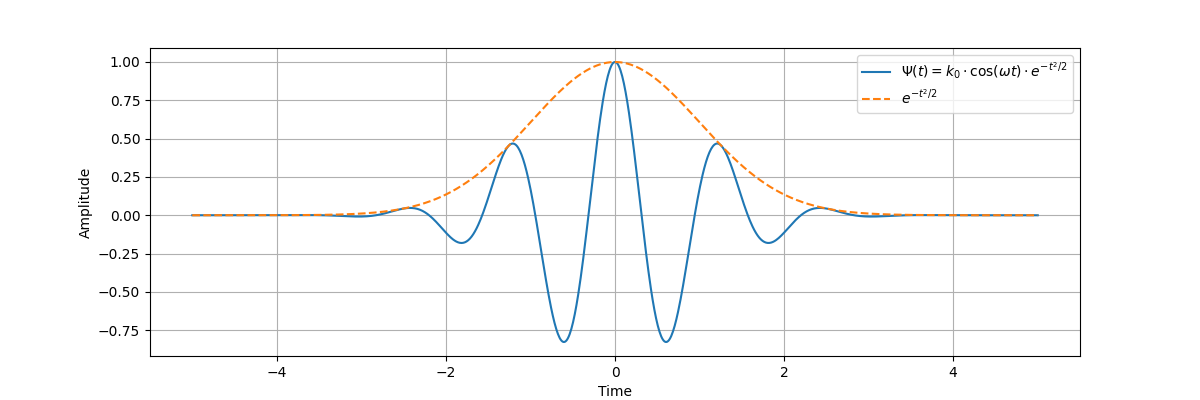
\includegraphics[width=\linewidth]{Rozdziały/02.Podstawy_teoretyczne/Obrazy/morlet_e}
        \caption{Falka Morlet (część rzeczywista)}
        \label{fig:image29}
    \end{minipage}
\end{figure}

Falka Morlet jest funkcją zespoloną, co oznacza, że składa się z części rzeczywistej i urojonej. Całość jest zdefiniowana następująco:
\begin{equation*}
    \Psi(t)=k e^{i \omega_0 t} \cdot e^{-\frac{t^2}{2}}
\end{equation*}

\begin{figure}[ht]
    \centering
    \begin{tikzpicture}[scale=0.8]
        \begin{axis}[
          ylabel={Re($\Psi$)},
          zlabel={Im($\Psi$)},
          xlabel={Czas},
          view={155}{30},
          colormap/viridis,
        ]
        \addplot3+[mesh, samples=30] table {Rozdziały/02.Podstawy_teoretyczne/Obrazy/wave_data.txt}; % Wczytanie danych
        \end{axis}
    \end{tikzpicture}
    \caption{Falka Morlet w przestrzeni 3D}
    \label{fig:image30}
\end{figure}

Inne funkcje falkowe:

\begin{figure}[ht]
    \centering
    \begin{minipage}[t]{0.3\linewidth}
        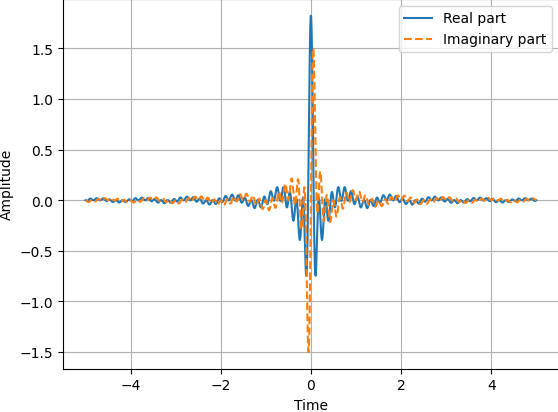
\includegraphics[width=\linewidth]{Rozdziały/02.Podstawy_teoretyczne/Obrazy/wavelet_fbsp1-1.5-1.0.png}
        \caption{Falka fbsp}
        \label{fig:image31}
    \end{minipage}
    \hspace{0.5cm}
    \begin{minipage}[t]{0.3\linewidth}
        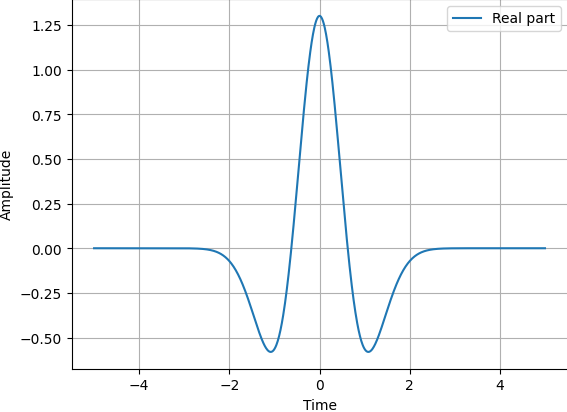
\includegraphics[width=\linewidth]{Rozdziały/02.Podstawy_teoretyczne/Obrazy/wavelet_mexh.png}
        \caption{Falka Mexican Hat}
        \label{fig:image32}
    \end{minipage}
    \hspace{0.5cm}
    \begin{minipage}[t]{0.3\linewidth}
        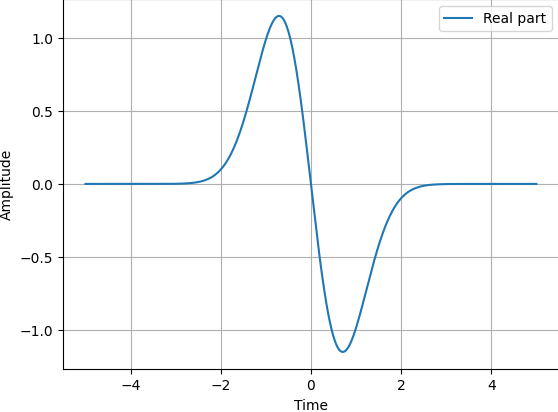
\includegraphics[width=\linewidth]{Rozdziały/02.Podstawy_teoretyczne/Obrazy/wavelet_gaus1.png}
        \caption{Falka Gaussa}
        \label{fig:image33}
    \end{minipage}
\end{figure}


\subsection*{Transformacja Falkowa}

Transformacja falkowa to proces dekompozycji sygnału na zestaw funkcji falkowych. W przeciwieństwie do transformacji Fouriera, która analizuje sygnał w kontekście czystych częstotliwości, transformacja falkowa rozkłada sygnał na serię "falek", które są przesuwane w czasie i częstotliwości, aby zbadać charakterystykę sygnału.


Transformację falkową przedstawiamy jako:

\begin{equation*}
    \tilde{s}_{\Psi}(a, b)=\frac{1}{\sqrt{a}} \int_{-\infty}^{\infty} s(t) \Psi\left(\frac{t-b}{a}\right) \mathrm{dt},
\end{equation*}

gdzie:
\begin{itemize}
    \item $s(t)$ - sygnał wejściowy,
    \item $\Psi\left(\frac{t-b}{a}\right)$ - funkcja falkowa,
    \item $b$ - parametr przesunięcia (w dziedzinie czasu) [Rys \ref{fig:image35}].
    \item $a$ - parametr skali (przesunięcie w dziedzinie częstotliwości) [Rys \ref{fig:image36}],
\end{itemize}


\begin{figure}[ht]
    \centering
    \begin{minipage}[t]{0.47\linewidth}
        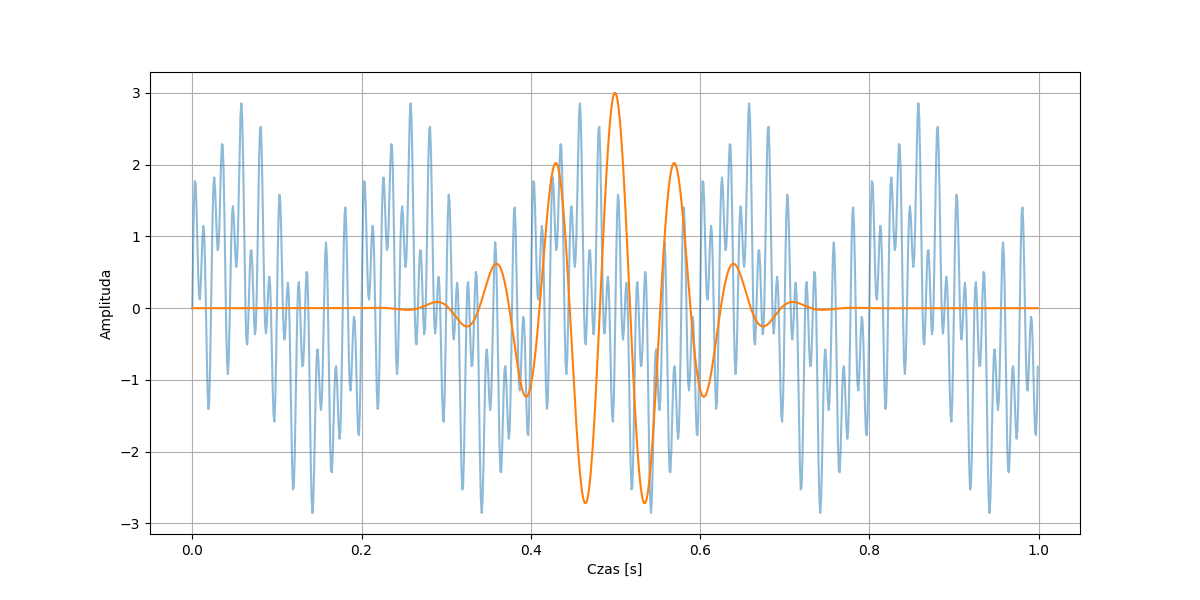
\includegraphics[width=\linewidth]{Rozdziały/02.Podstawy_teoretyczne/Obrazy/morlet_bez_przesuniecia.png}
        \caption{Brak przesunięcia}
        \label{fig:image34}
    \end{minipage}
    \centering
    \begin{minipage}[t]{0.47\linewidth}
        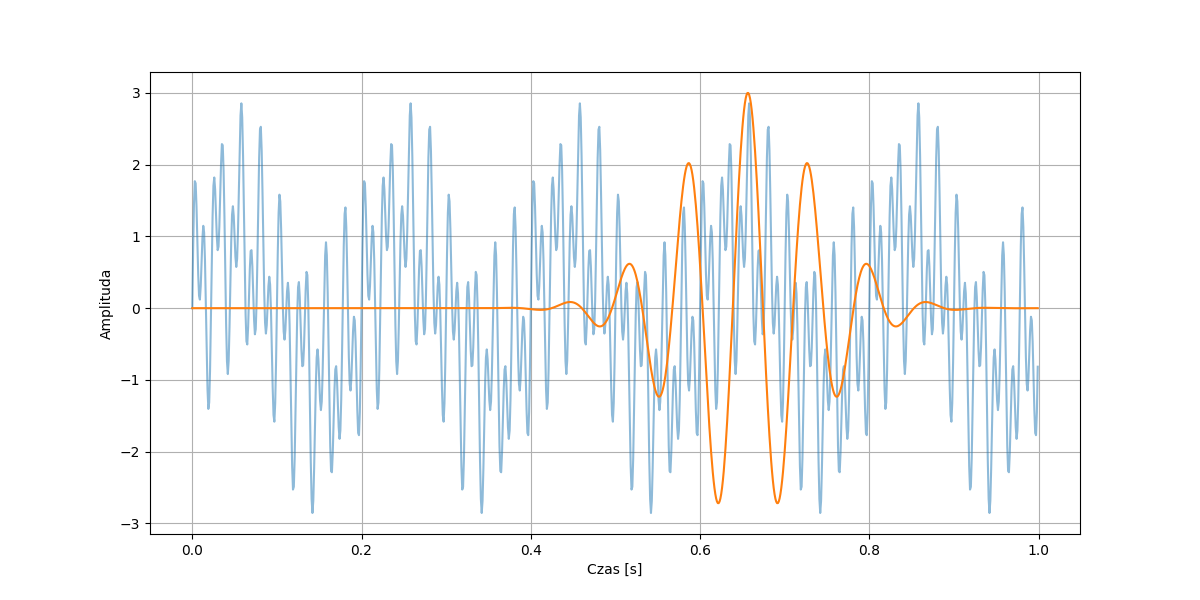
\includegraphics[width=\linewidth]{Rozdziały/02.Podstawy_teoretyczne/Obrazy/time_shift_morlet.png}
        \caption{Przesunięcie w czasie}
        \label{fig:image35}
    \end{minipage}
\end{figure}

\begin{figure}[ht]
    \centering
    \begin{minipage}[t]{0.46\linewidth}
        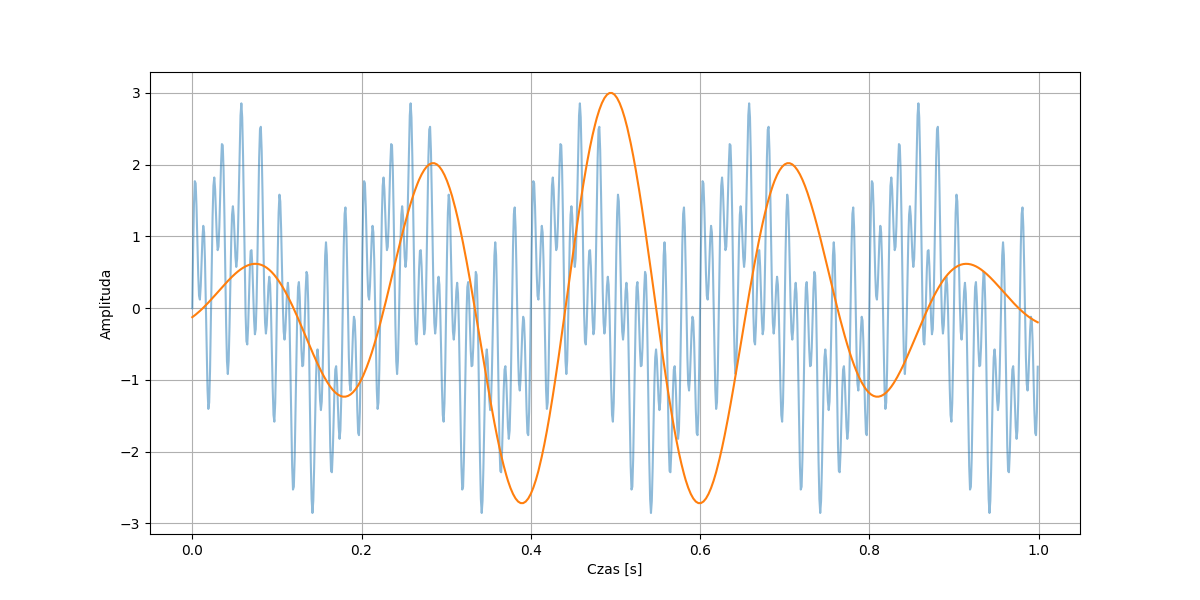
\includegraphics[width=\linewidth]{Rozdziały/02.Podstawy_teoretyczne/Obrazy/f_shift_morlet.png}
        \caption{Przesunięcie w częstotliwości}
        \label{fig:image36}
    \end{minipage}
    \centering
    \begin{minipage}[t]{0.46\linewidth}
        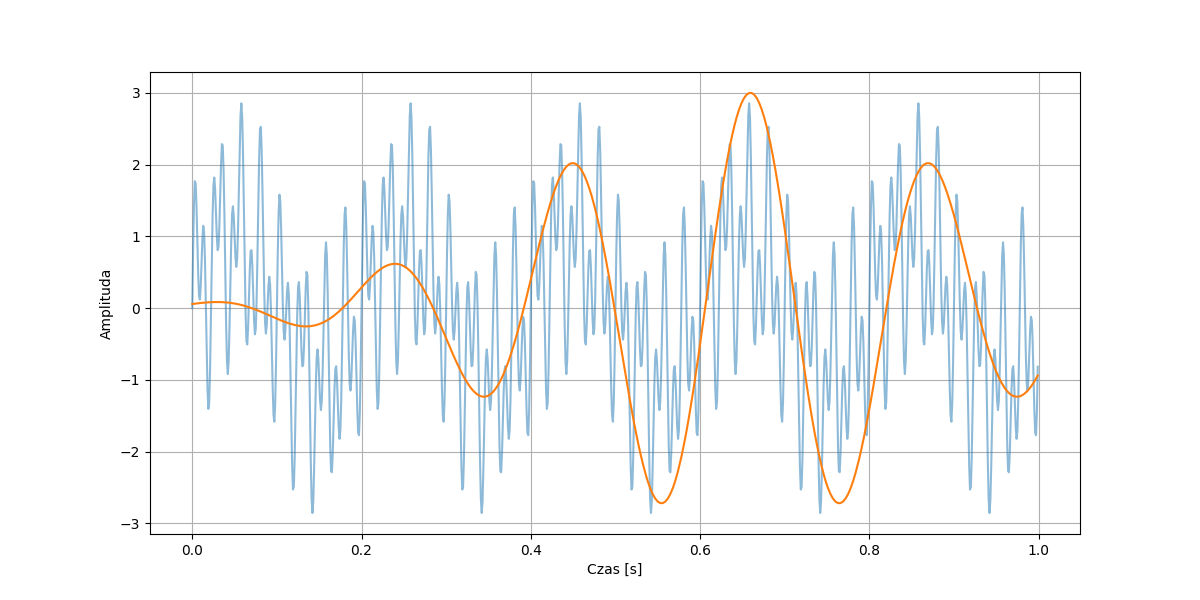
\includegraphics[width=\linewidth]{Rozdziały/02.Podstawy_teoretyczne/Obrazy/t_and_f_shift_morlet.png}
        \caption{Przesunięcie w $t$ i $f$}
        \label{fig:image37}
    \end{minipage}
\end{figure}


Wynikiem transformacji falkowej jest mapa współczynników, które są zależne od parametrów $a$ i $b$, wybranej funkcji falkowej oraz sygnału wejściowego. Dla danych wartości $a$ i $b$ współczynnik jest miarą podobieństwa pomiędzy falką a fragmentem sygnału. Im większa wartość współczynnika, tym większe podobieństwo.

% \begin{equation*}
%     T\left(a,b\right) = \int_{-\infty}^{+\infty} y(t) \cdot \Psi_{a, b}(t) d t
% \end{equation*}

W rezultacie funkcja $ \tilde{s}_{\Psi}\left(a,b\right)$ składa się na mapę współczynników, która jest reprezentacją sygnału w dziedzinie czasu i częstotliwości. Mapę taką nazywamy skalogramem, skalogram przykładowego sygnału przedstawiono na Rys \ref{fig:image38} i \ref{fig:image39}.

\begin{figure}[ht]
    \centering
    \begin{minipage}[t]{0.9\linewidth}
        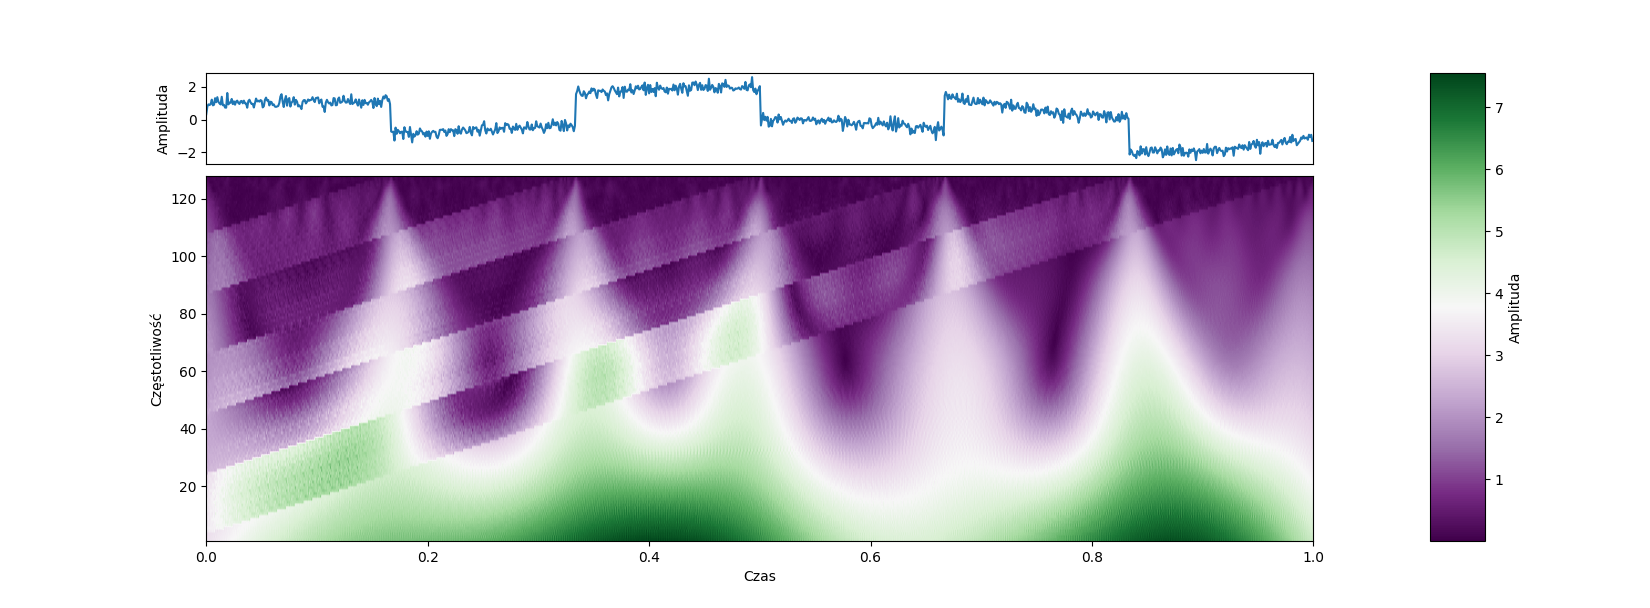
\includegraphics[width=\linewidth]{Rozdziały/02.Podstawy_teoretyczne/Obrazy/skalogram.png}
        \caption{Skalogram falkowy w zestawieniu z sygnałem wejściowym}
        \label{fig:image38}
    \end{minipage}
\end{figure}

\begin{figure}[ht]
    \centering
    \begin{tikzpicture}[scale=0.95]
        \begin{axis}[
          xlabel={Czas},
          ylabel={Częstotliwość},
          zlabel={Amplituda},
          view={-40}{40},
          colormap/viridis,
          yticklabel=\empty,            % Hide y-axis numbers
          xticklabel=\empty,            % Hide x-axis numbers
          zticklabel=\empty,            % Hide z-axis numbers
        ]
        \addplot3[surf] file {Rozdziały/02.Podstawy_teoretyczne/Obrazy/wavelet_coefficients_magnitude.txt};
        \end{axis}
    \end{tikzpicture}
    \caption{Skalogram falkowy w przestrzeni 3D}
    \label{fig:image39}
\end{figure}
\newpage
Rozdzielczość czasu i rozdzielczości w transformacji falkowej nie jest idealna, widać że mamy do czynienia z kompromisem pomiędzy tymi wartościami, szczególnie przy analizy zwykłej funkcji sinus. Skalogram dla sinusa [Rys \ref{fig:image40}] nie przedstawia jednoznacznie częstotliwości sygnału, jest to jedynie przybliżenie co widać na krawędziach skalogramu.

\begin{figure}[ht]
    \centering
    \begin{minipage}[t]{0.55\linewidth}
        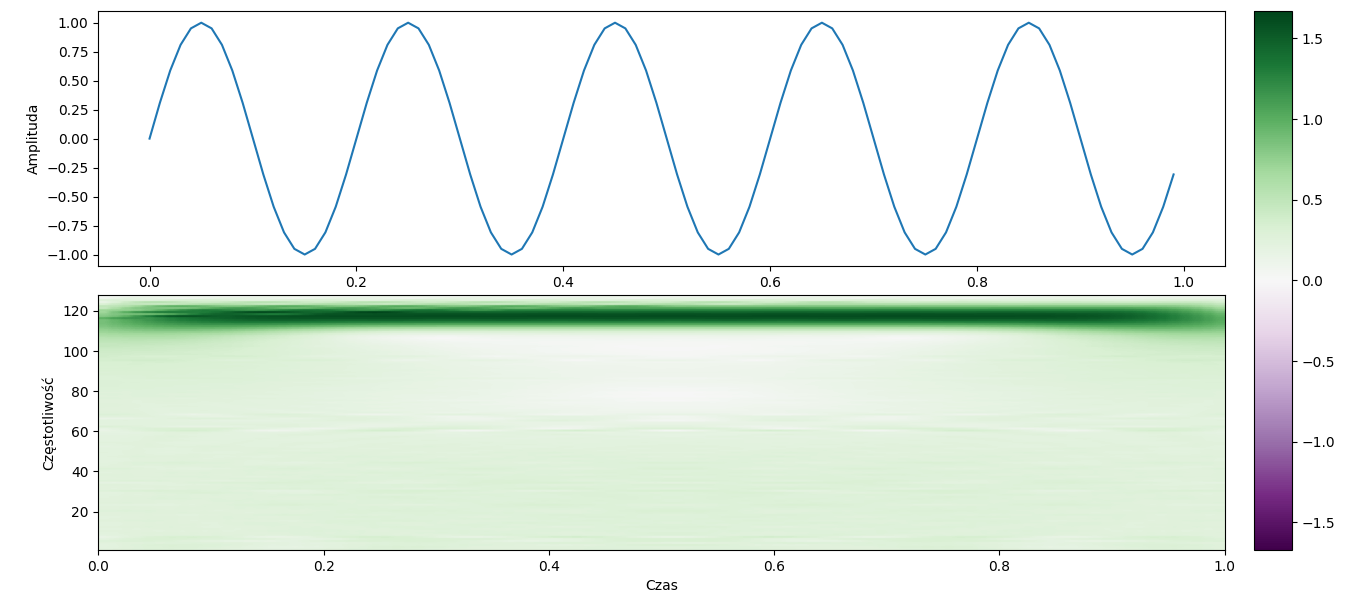
\includegraphics[width=\linewidth]{Rozdziały/02.Podstawy_teoretyczne/Obrazy/skalogram_sinus.png}
        \caption{Niedokładność danych na skalogramie}
        \label{fig:image40}
    \end{minipage}
\end{figure}

\newpage
\subsubsection{Dyskretna Transformacja Falkowa}

Dyskretna transformacja falkowa (DWT) jest dyskretną wersją transformacji falkowej, czyli działa na dyskretnych danych wejściowych. Przykładem takich danych może być cyfrowy sygnał taki jak obraz lub dźwięk. 

Dla sygnałów dyskretnych, transformacja falkowa jest zdefiniowana jako:
\begin{equation*}
    \mathrm{D}\left(m, a^j\right)=\frac{1}{\sqrt{a^j}} \sum_{n=0}^{N-1} x\varphi^*[n] \left(\frac{n-m}{a^j}\right),
\end{equation*}
gdzie:
\begin{itemize}
    \item $x[n]$ - sygnał dyskretny,
    \item $\varphi[n]$ - dyskretna funkcja falkowa,
    \item $a$ - parametr skali,
    \item $j$ - poziom dekompozycji,
    \item $N$ - liczba próbek sygnału,
    \item $m$ - indeks próbki.
\end{itemize}

Aby wykonać dyskretną transformację falkową sygnał $x[n] \in \mathbb{R}^N$ jest przepuszczany przez filtr górnoprzepustowy $G_H[n]$ i filtr dolnoprzepustowy $G_L[n]$, które są definiowane jako (w przypadku falki Haara):

\begin{equation*}
    G_H[n]=\left\{\begin{array}{ll}
    1, & n=0 \\
    -1, & n=1 \\
    0, & \text {w przeciwnym razie}
    \end{array}, 
    G_L[n]= \begin{cases}1, & n=0,1 \\
    0, & \text {w przeciwnym razie}\end{cases}\right.
\end{equation*}

Po filtrowaniu połowa próbek może zostać wyeliminowana zgodnie z regułą Nyquista, ponieważ sygnał ma teraz pasmo częstotliwości $\frac{\pi}{2}$ radianów zamiast $/pi$.

Obraz $x$ jest reprezentowany jako sygnał $2 D$ o indeksach $[n,m]$, gdzie $x[n,m]$ jest wartością piksela w $n$-tej kolumnie i $m$-tym wierszu.

Sygnał dwuwymiarowy $x[n,m]$ może być traktowany jako dwa sygnały jednej zmiennej: $x[n,:]$ w $n$-tej kolumnie i wśród kolumn $x[:,m]$ w $m$-tym wierszu. Transformacja falkowa o pierwszym stopniu dekompozycji może być wykonywana w sposób przedstawiony na Rys \ref{fig:image41}.

\begin{figure}[ht]
    \centering
    \begin{minipage}[t]{0.6\linewidth}
        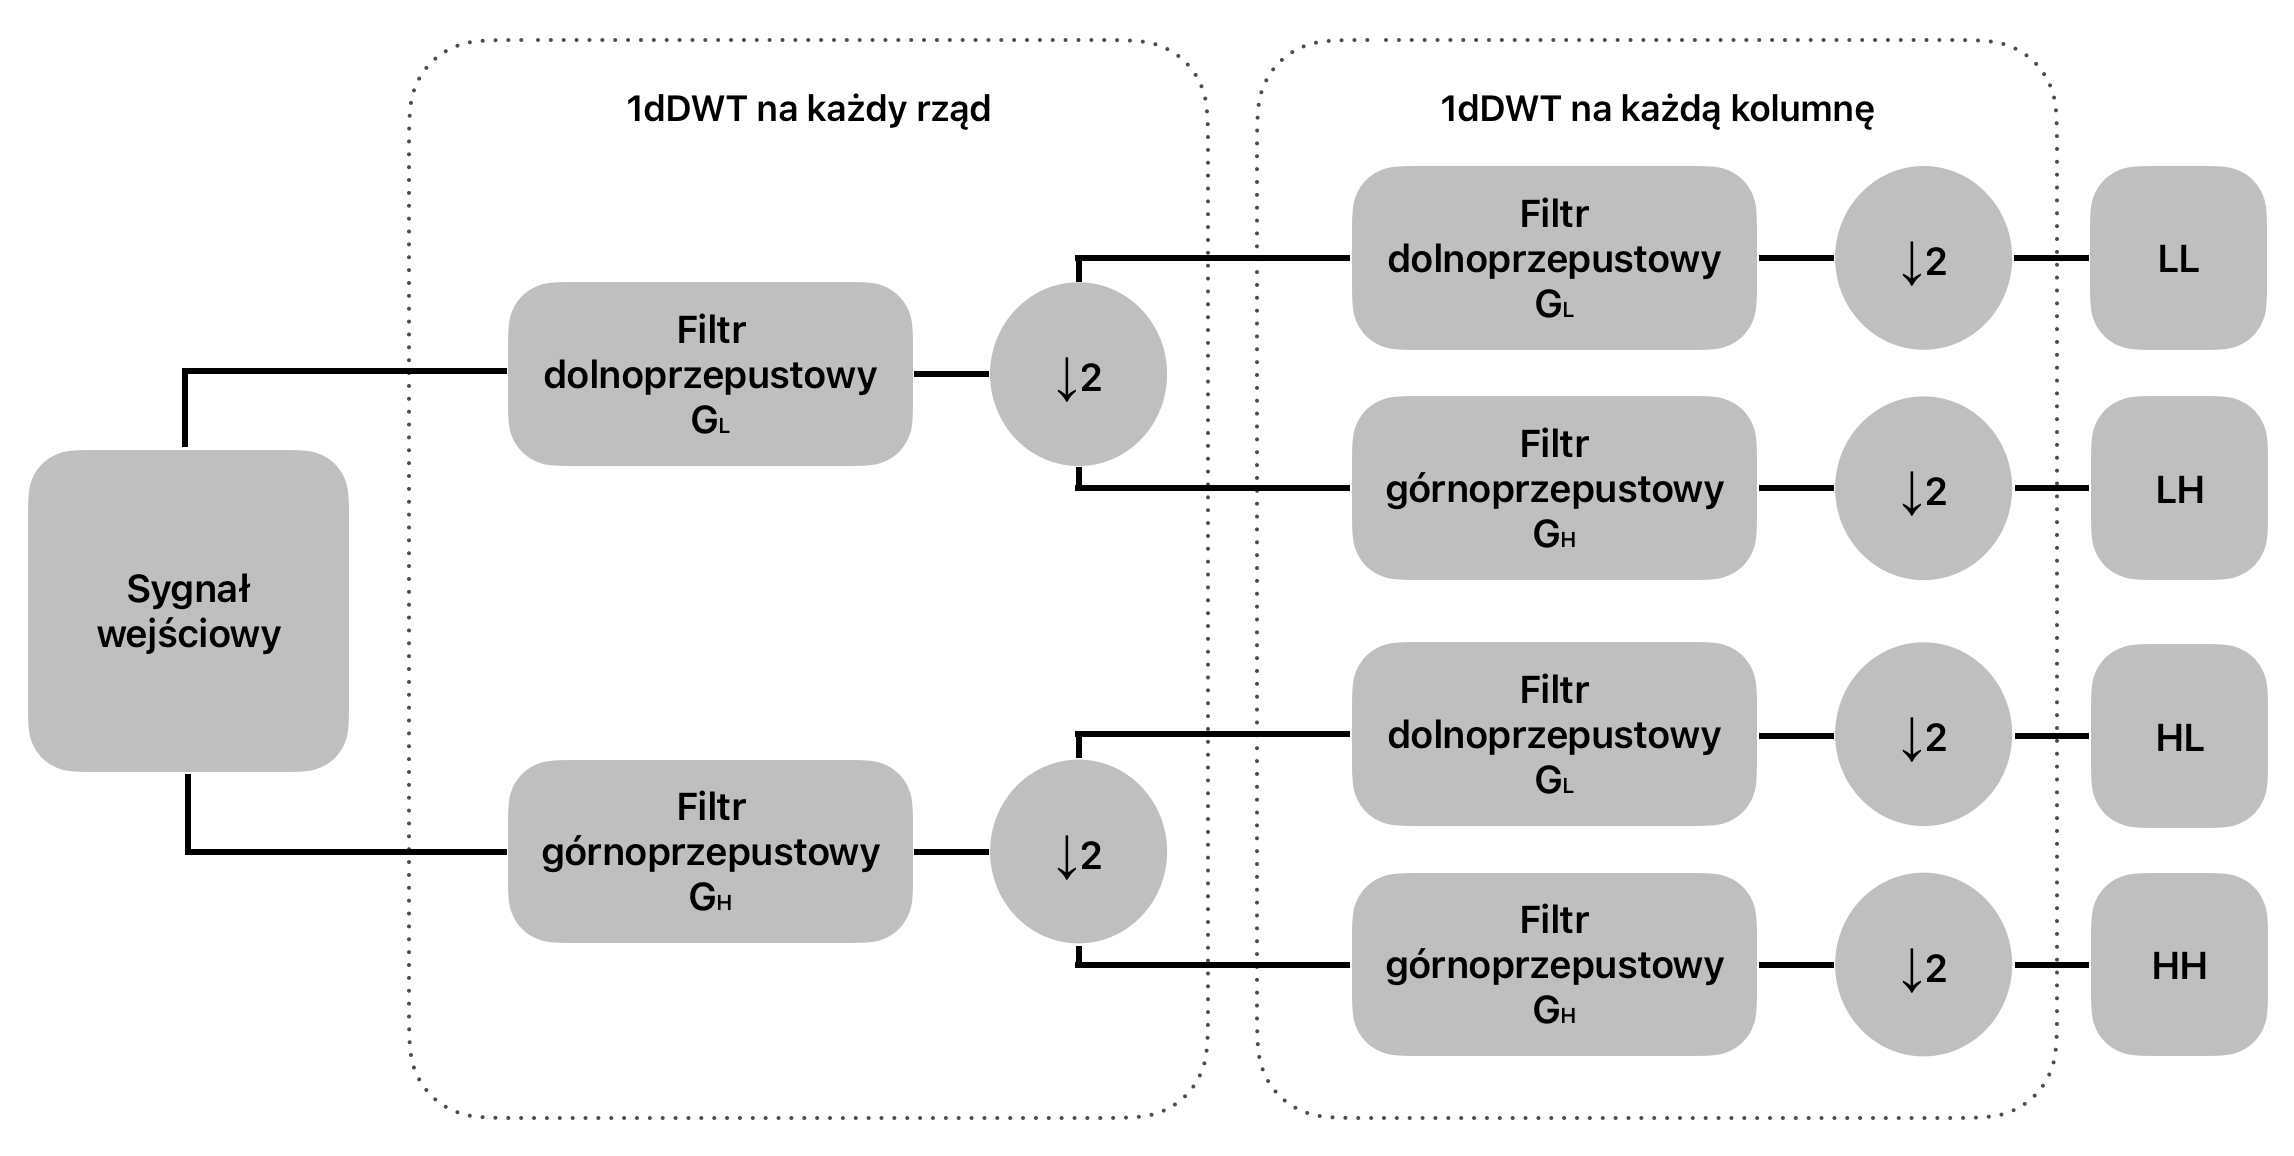
\includegraphics[width=\linewidth]{Rozdziały/02.Podstawy_teoretyczne/Obrazy/DWT_dekompozycja.png}
        \caption{Dekompozycja DWT 1-poziomu}
        \label{fig:image41}
    \end{minipage}
\end{figure}

Przykładowa dekompozycja pierwszego stopnia wykonana na obrazie \textbf{comic.png} widoczna jest na Rys \ref{fig:image42} - niskie częstotliwości na obrazie, \ref{fig:image43} - poziome detale, \ref{fig:image44} - pionowe detale, \ref{fig:image45} - detale diagonalne. Obrazy po dekompozycji są tej samej wielkości co obraz wejściowy. 

Jeśli chcemy wykonać odwrotną transformację falkową na obrazie, wystarczy wykonać kroki z Rys \ref{fig:image41}. 


\begin{figure}[ht]
    \centering
    \begin{minipage}[t]{0.35\linewidth}
        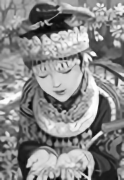
\includegraphics[width=\linewidth]{Rozdziały/02.Podstawy_teoretyczne/Obrazy/level_1_decomposition_LL.png}
        \caption{LL (niskie częstotliwości)}
        \label{fig:image42}
    \end{minipage}
    \centering
    \begin{minipage}[t]{0.35\linewidth}
        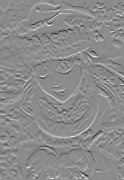
\includegraphics[width=\linewidth]{Rozdziały/02.Podstawy_teoretyczne/Obrazy/level_1_decomposition_LH.png}
        \caption{LH (poziome detale)}
        \label{fig:image43}
    \end{minipage}
\end{figure}

\begin{figure}[ht]
    \centering
    \begin{minipage}[t]{0.35\linewidth}
        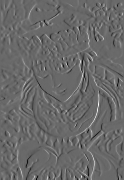
\includegraphics[width=\linewidth]{Rozdziały/02.Podstawy_teoretyczne/Obrazy/level_1_decomposition_HL.png}
        \caption{HL (pionowe detale)}
        \label{fig:image44}
    \end{minipage}
    \centering
    \begin{minipage}[t]{0.35\linewidth}
        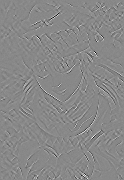
\includegraphics[width=\linewidth]{Rozdziały/02.Podstawy_teoretyczne/Obrazy/level_1_decomposition_HH.png}
        \caption{HH (diagonalne detale)}
        \label{fig:image45}
    \end{minipage}
\end{figure}


 
% \chapter{DWSR: Deep Wavelet Super Resolution}


\section{Architektura DWSR}


Dokładne przedstawienie struktury i funkcjonowania sieci DWSR, podkreślając jej unikalne cechy i mechanizmy.


\section{Kluczowe cechy i innowacje}


Dyskusja na temat głównych innowacyjnych rozwiązań zastosowanych w DWSR i ich wpływu na efektywność metody.


\section{Proces treningu i implementacji}


Wyjaśnienie procedur związanych z treningiem DWSR, z uwzględnieniem specyfikacji danych, procesu uczenia i kwestii implementacji.


\section{Przykłady zastosowań i rezultaty}


Ilustracja praktycznych zastosowań DWSR oraz ocena i interpretacja osiągniętych dzięki niemu wyników.

% \chapter{Enhanced Super-Resolution Generative Adversarial Network} \label{chap:ESRGAN}

Kolejny omawiany algorytm rozwiązuje problem super-rozdzielczości obrazów przy użyciu Generatywnych Sieci Przestawnych. Algorytm został opracowany przez: Xintao Wang, Ke Yu, Shixiang Wu, Jinjin Gu, Yihao Liu,
Chao Dong, Chen Change Loy, Yu Qiao, Xiaoou Tang \cite{wang2018esrgan}.

\textbf{ESRGAN} jest rozwinięciem algorytmu \textbf{SRGAN} \cite{Ledig_2017_CVPR}; wprowadza kilka istotnych zmian, które znacznie poprawiają jakość obrazów wygenerowanych przez sieć. W tej pracy badane są zalety zastosowanych zmian w architekturze sieci generatora i dyskryminatora, oraz funkcji straty. 


\begin{figure}[ht]
    \centering
    \begin{minipage}[t]{0.4\linewidth}
        
\includegraphics[width=\linewidth]{Rozdziały/02.Podstawy_teoretyczne/Obrazy/comic.png}
        \caption{Obraz wejściowy}
        \label{fig:image60}
    \end{minipage}
    \hspace{0.5cm}
    \begin{minipage}[t]{0.4\linewidth}
        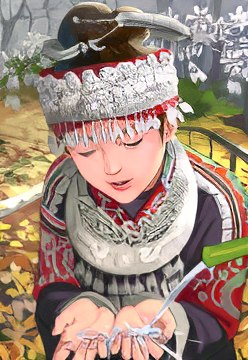
\includegraphics[width=\linewidth]{Rozdziały/02.Podstawy_teoretyczne/Obrazy/comic_ESRGAN_x4.png}
        \caption{Obraz powiększony algorytmem \textbf{ESRGAN} czterokrotnie}
        \label{fig:image61}
    \end{minipage}
\end{figure}

\newpage
\section{Architektura ESRGAN}

Algorytm \textbf{ESRGAN} bazuje na założeniach \textbf{SRGAN} \cite{Ledig_2017_CVPR}, jednak wprowadza istotne zmiany w architekturze sieci, przeciwnych strat i strat percepcyjnych.

\begin{figure}[ht]
    \centering
    \begin{minipage}[t]{0.85\linewidth}
        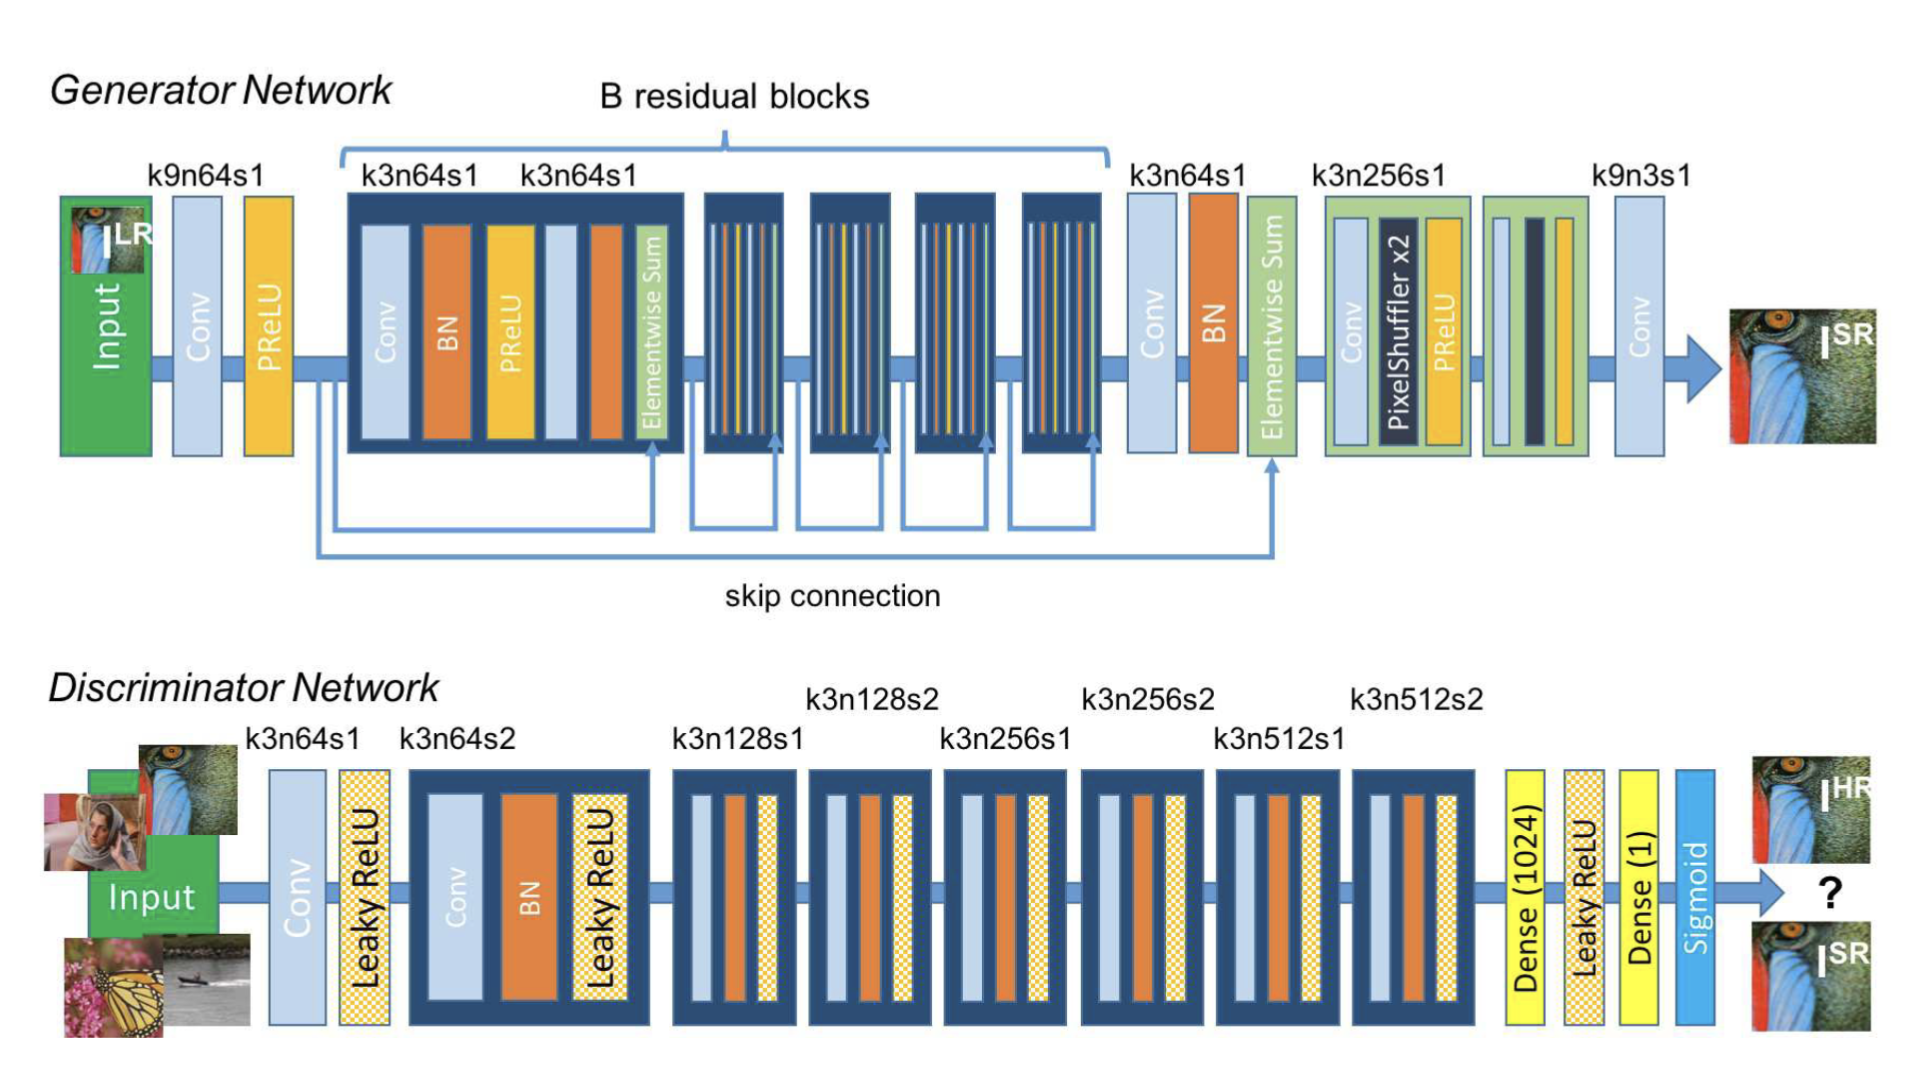
\includegraphics[width=\linewidth]{Rozdziały/04.ESRGAN/Obrazy/Architektura SRGAN.png}
        \caption{Architektura \textbf{SRGAN}}
        \label{fig:image62}
    \end{minipage}
\end{figure}

Architektura \textbf{SRGAN} składa się z dwóch sieci: generatora i dyskryminatora [Rys \ref{fig:image62}]. Generator przyjmuje na wejściu obraz o niskiej rozdzielczości i zwraca obraz o wysokiej rozdzielczości. Dyskryminator przyjmuje na wejściu obraz o wysokiej rozdzielczości i zwraca prawdopodobieństwo, że obraz jest rzeczywisty, a nie wygenerowany przez sieć. 

\textbf{SRGAN} wykorzystuje VGG loss, czyli funkcję straty opartą na głębokiej sieci neuronowej VGG, używaną do oceny podobieństwa percepcyjnego między obrazami. Zamiast mierzyć różnicę pomiędzy pikselami, jak w przypadku błędu średniokwadratowego (MSE), VGG loss porównuje cechy reprezentacyjne (np. tekstury, kształty) wyekstrahowane przez sieć VGG z obu obrazów. Poprzez użycie tej funkcji straty, SRGAN skupia się na generowaniu obrazów, które są percepcyjnie bardziej podobne do obrazów wysokiej rozdzielczości, zamiast jedynie minimalizować błąd średniokwadratowy. Dzięki temu, generowane obrazy charakteryzują się lepszą jakością percepcyjną, bardziej zbliżoną do naturalnych zdjęć.



\textbf{ESRGAN} wprowadza kilka istotnych zmian w architekturze sieci. Zmiany te mają na celu poprawę jakości generowanych obrazów i eliminację artefaktów na obrazach wyjściowych.


\subsection*{Zmiany w architekturze}

\begin{figure}[ht]
    \centering
    \begin{minipage}[t]{0.85\linewidth}
        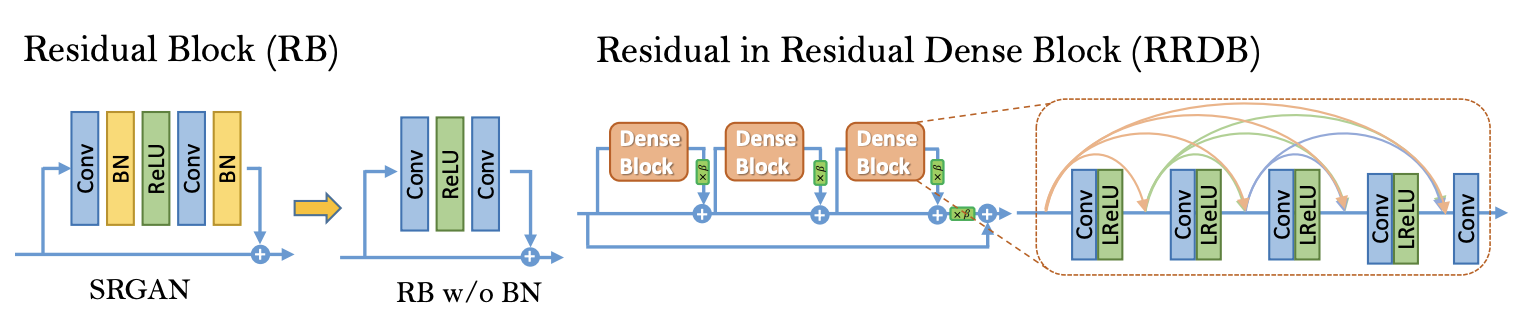
\includegraphics[width=\linewidth]{Rozdziały/04.ESRGAN/Obrazy/Architektura ESRGAN 1.png}
        \caption{Zmiany zastosowane w architekturze \textbf{ESRGAN}}
        \label{fig:image63}
    \end{minipage}
\end{figure}

Pierwszą zmianą było usunięcie warstw normalizacji wsadowej z generatora (lewa strona Rys \ref{fig:image63}). 
Normalizacja wsadowa jest techniką stosowaną w procesie uczenia sieci neuronowych, która ma na celu poprawę stabilności i szybkości uczenia poprzez normalizację danych wejściowych w każdej warstwie na podstawie mini-zestawów (batchy). Technika ta polega na dostosowaniu średniej i wariancji danych w każdym mini-zestawie, co pomaga w redukcji problemu zwanego "wewnętrznym przesunięciem kowariancji" (internal covariance shift) i sprzyja szybszemu i bardziej stabilnemu uczeniu sieci.

Warstwy te powodowały, że obrazy wyjściowe posiadały artefakty [Rys \ref{fig:image64}] - powtarzające się tekstury.

\begin{figure}[ht]
    \centering
    \begin{minipage}[t]{0.85\linewidth}
        \includegraphics[width=\linewidth]{Rozdziały/04.ESRGAN/Obrazy/Batch normalization artefacts.png}
        \caption{Przykłady artefaktów powstałych przez normalizację wsadową}
        \label{fig:image64}
    \end{minipage}
\end{figure}

Kolejną zmianą było powiększenie ilości warstw w generatorze (prawa strona Rys \ref{fig:image63}). W \textbf{SRGAN} generator składał się z 16 warstw, natomiast w \textbf{ESRGAN} z 23 warstw. Zwiększenie ilości warstw pozwoliło na zwiększenie złożoności sieci, co przełożyło się na lepszą jakość generowanych obrazów.

\subsection*{Zmiany w dyskryminatorze}

W \textbf{ESRGAN} zastosowano zmiany nie tylko w generatorze, ale również w dyskryminatorze stosując dyskryminator relatywistyczny \cite{jolicoeurmartineau2018relativistic}. Dyskryminator stosowany w \textbf{SRGAN} zwracał prawdopodobieństwo, że obraz jest rzeczywisty, a nie wygenerowany przez sieć. Dyskryminator relatywistyczny przewiduje prawdopodobieństwo czy obraz prawdziwy jest relatywnie bardziej realistyczny niż obraz wygenerowany przez generator [Rys \ref{fig:image66}].

\begin{figure}[ht]
    \centering
    \begin{minipage}[t]{0.85\linewidth}
        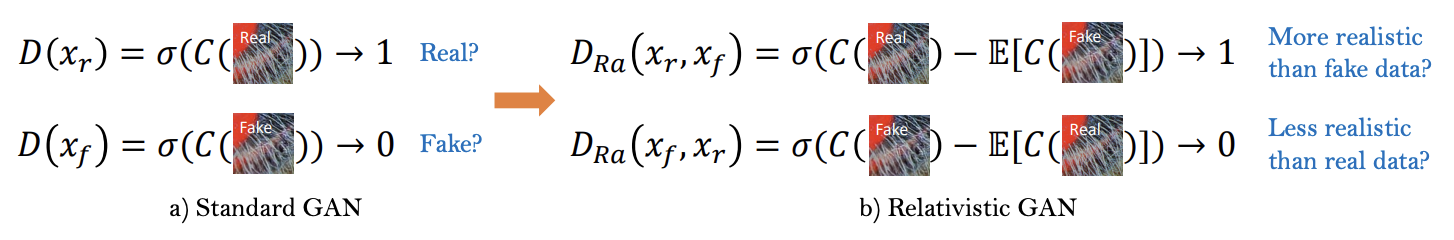
\includegraphics[width=\linewidth]{Rozdziały/04.ESRGAN/Obrazy/relatywistyczny dyskryminator.png}
        \caption{Różnica między dyskryminatorem standardowym a relatywistycznym}
        \label{fig:image66}
    \end{minipage}
\end{figure}

\subsection*{Zmiany w funkcji straty}

Zastosowano również zmianę w funkcji straty. Zastosowano funkcję strat VGG, ale mapy cech były porównywane przed aktywacją, a nie po. Porównanie cech przed aktywacją pozwala wykorzystanie większej ilości informacji, gdyż mapy aktywacji są gęstsze i zawierają więcej informacji o obrazie przed analizą przez funkcję aktywacji [Rys \ref{fig:image65}].

\begin{figure}[ht]
    \centering
    \begin{minipage}[t]{0.85\linewidth}
        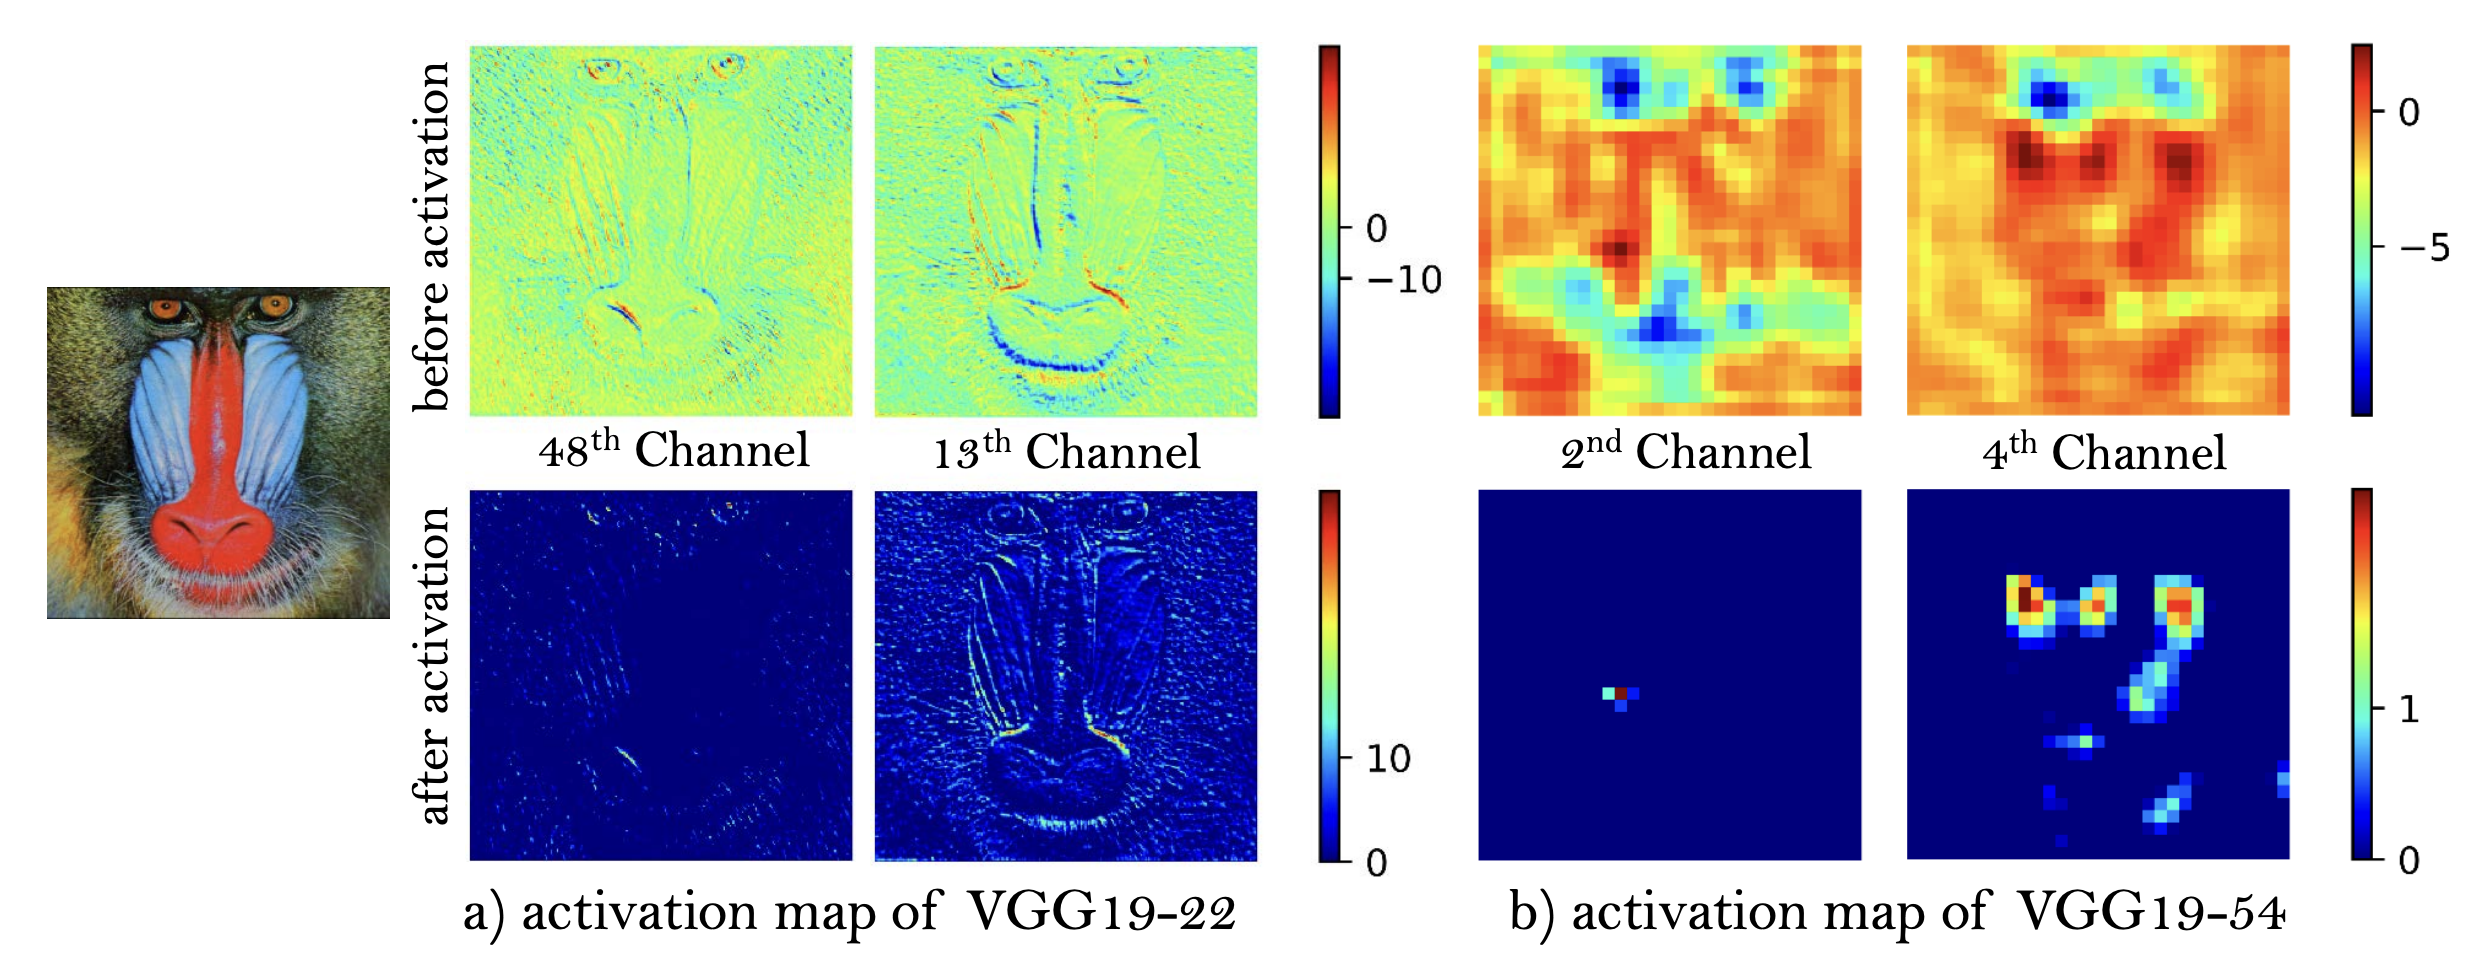
\includegraphics[width=\linewidth]{Rozdziały/04.ESRGAN/Obrazy/mapa aktywacji.png}
        \caption{Mapa cech przed aktywacją i po aktywacji}
        \label{fig:image65}
    \end{minipage}
\end{figure}



\section{Proces treningu}

Podobnie jak w \textbf{SRGAN} \cite{Ledig_2017_CVPR}, w \textbf{ESRGAN} \cite{wang2018esrgan} obrazy powiększane są ze skalą 4 pomiędzy obrazami $LR$ a $HR$. 

Do treningu \textbf{ESRGAN} wykorzystano bazę danych DIV2K \cite{Agustsson_2017_CVPR_Workshops}, która zawiera 800 zdjęć o wysokiej rozdzielczości (2k), oraz zbioru danych Flickr2K % \cite{lim2017enhanced}
, który zawiera 2650 zdjęć o takiej samej rozdzielczości. Dodatkowo wzbogacono zestaw treningowy o losowe odbicia lustrzane i rotacje o 90 stopni.


Obrazy $HR$ przeskalowano z użyciem Matlaba. Używano mini-zestawów (mini-batch) o wielkości 16 i kadrowano fragmenty HR o rozmiarze $128 \times 128$ pikseli. Większy rozmiar fragmentów pomagał w przechwytywaniu większej ilości informacji semantycznej, co było korzystne dla głębszych sieci, ale zwiększało czas treningu i zapotrzebowanie na zasoby obliczeniowe.

Do optymalizacji użyto metody Adam z parametrami \( \beta_1 = 0.9 \) i \( \beta_2 = 0.999 \), aktualizując na przemian sieci generatora i dyskryminatora do momentu zbieżności modelu.

Jako zestaw testowy wykorzystano obrazy z zestawów danych Set5 \cite{bevilacqua2012low}, Set14 \cite{zeyde2010single}, BSD100 \cite{martin2001database} i Urban100 \cite{Huang_2015_CVPR}.



\section{Przykłady zastosowań i rezultaty}

Przykładowe wyniki działania algorytmu \textbf{ESRGAN} przedstawiono na Rys: \ref{fig:image68} \ref{fig:image70}, \ref{fig:image72}. Obrazy pochodzą z repozytorium GitHub, gdzie umieszczony został również algorytm \textbf{DWSR} \cite{guo2017deep}.

Omawiany algorytm radzi sobie jeszcze lepiej niż opisywany w poprzednim rozdziale \textbf{DWSR}, zwłaszcza z teksturami takimi jak włosy, czy futro. \textbf{ESRGAN} świetnie radzi sobie z krawędziami obiektów na obrazach, widać to na przykładzie Rys. \ref{fig:image70}, gdzie ramy okien są bardzo wyraźnie zarysowane.

Jako, że \textbf{ESRGAN} jest dużym i skomplikowanym modelem jego czas egzekucji jest znacznie dłuższy niż w przypadku \textbf{DWSR}. 

Dokładniejsza analiza działania algorytmu \textbf{ESRGAN}, oraz analiza porównawcza z algorytmem \textbf{DWSR} została przedstawiona w Rozdziale \ref{chap:porownanie_algorytmow}.


\begin{figure}[ht]
    \centering
    \begin{minipage}[t]{0.45\linewidth}
        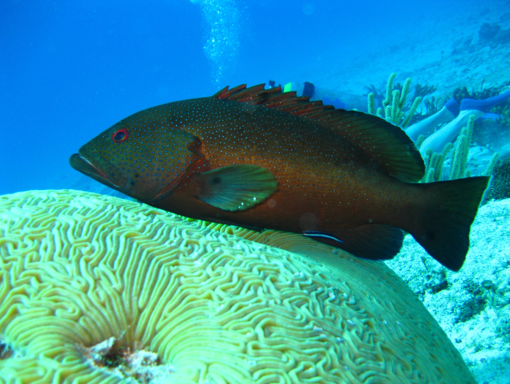
\includegraphics[width=\linewidth]{Rozdziały/03.DWSR/Obrazy/0904x4.png}
        \caption{Obraz wejściowy}
        \label{fig:image67}
    \end{minipage}
    \hspace{0.5cm}
    \begin{minipage}[t]{0.45\linewidth}
        \includegraphics[width=\linewidth]{Rozdziały/03.DWSR/Obrazy/0904x4_ESRGANx4.png}
        \caption{Obraz powiększony algorytmem \textbf{ESRGAN} czterokrotnie}
        \label{fig:image68}
    \end{minipage}
\end{figure}

\begin{figure}[ht]
    \centering
    \begin{minipage}[t]{0.45\linewidth}
        \includegraphics[width=\linewidth]{Rozdziały/03.DWSR/Obrazy/0913x4.png}
        \caption{Obraz wejściowy}
        \label{fig:image69}
    \end{minipage}
    \hspace{0.5cm}
    \begin{minipage}[t]{0.45\linewidth}
        \includegraphics[width=\linewidth]{Rozdziały/03.DWSR/Obrazy/0913x4_ESRGANx4.png}
        \caption{Obraz powiększony algorytmem \textbf{ESRGAN} czterokrotnie}
        \label{fig:image70}
    \end{minipage}
\end{figure}

\begin{figure}[ht]
    \centering
    \begin{minipage}[t]{0.45\linewidth}
        \includegraphics[width=\linewidth]{Rozdziały/03.DWSR/Obrazy/0999x4.png}
        \caption{Obraz wejściowy}
        \label{fig:image71}
    \end{minipage}
    \hspace{0.5cm}
    \begin{minipage}[t]{0.45\linewidth}
        \includegraphics[width=\linewidth]{Rozdziały/03.DWSR/Obrazy/0999x4_ESRGANx4.png}
        \caption{Obraz powiększony algorytmem \textbf{ESRGAN} czterokrotnie}
        \label{fig:image72}
    \end{minipage}
\end{figure}
% \chapter{Aplikacja webowa do powiększania rozdzielczości obrazów} \label{chap:app}

Podczas korzystania z Internetu miałem kilka sytuacji w których potrzebowałem narzędzia, które pozwoli mi na powiększenie rozdzielczości obrazów. Stron internetowych tego typu jest wiele, sporo aplikacji do edycji zdjęć umożliwia powiększenie rozdzielczości obrazów, przykładem może być \textbf{Photoshop} i inne.

Korzystając z rozwiązań ogólnodostępnych zauważyłem, że darmowe aplikacje nie gwarantują wysokiej jakości obrazów wyjściowych, zaś bardziej rozbudowane rozwiązania są płatne lub mają dostępne tylko jedno powiększenie obrazu na dobę. 

Postanowiłem więc wykorzystac ogólnodostępne algorytmy rozwiązujące problem super-rozdzielczości, następnie użyć ich do aplikacji która w domyśle będzie darmowa i będzie dawała możliwość porównania wyników działania kilku algorytmów. Nie zawsze jedna z wdrożonych metod będzie dawać najlepsze wyniki, więc chciałbym żeby użytkownik miał wybór a pro po tego którą metodę chce wykorzystać.

Głównym założeniem aplikacji jest intuicyjność i minimalizacja interakcji potrzebnych do powiększenia obrazu; zauważyłem, że rozwiązania konkurencji wymagają akceptacji regulaminów, lub dopiero po przejściu kilku ekranów możemy wysłać obraz, którego rozdzielczość chcemy powiększyć. Uznałem to za bardzo ważne, gdyż użytkownicy chcą szybko dostać wynik, użytkownik nie będzie czekał nie wiadomo jak długo na wynik.

Nie spotkałem się z tym, żeby aplikacje innych firm pozwalały na porównanie wyników różnych algorytmów ze sobą. Uważam że to jest istotne gdy chcemy uzyskać wynik najwyższej jakości, bo jak wspomniałem nie ma rozwiązań idealnych i nie zawsze jedna z wdrożonych metod będzie dawać najlepsze wyniki.

Ważne jest dla mnie, żeby aplikacja była estetyczna i przyjemna dla oka. Dużo chętniej korzystamy z narzędzi czy urządzeń które lepiej wyglądają, bardziej się nam podobają i chciałbym żeby tak było w tym przypadku. W planie również jest dbanie o animacje i o to żeby interakcje z narzędziem były przyjemne i satysfakcjonujące.

\newpage
\begin{figure}[H]
    \begin{minipage}{\linewidth}
        \centering
        \includegraphics[width=\linewidth]{Rozdziały/06.Aplikacja/Obrazy/kursor-link.jpg}  
        \caption{Widok strony głównej aplikacji}
        \label{fig:image80}
        \hspace{2cm}
        \includegraphics[width=\linewidth]{Rozdziały/06.Aplikacja/Obrazy/display5.jpg}  
        \caption{Widok prezentacji wyników}
        \label{fig:image81}
    \end{minipage}
\end{figure}
\newpage

\section{Projektowanie aplikacji}

Pierwszym etapem tworzenia aplikacji było stworzenie diagramu przepływu użytkownika (user flow diagram) [Rys \ref{fig:image82}], który ilustruje kolejność interakcji użytkownika z aplikacją. Potencjalni użytkownicy mają już pewne oczekiwania i potrzeby, spodziewają się gdzie na ekranie znajdą się konkretne elementy. Dlatego ważne jest, żeby zrozumieć jak użytkownik będzie korzystał z aplikacji, jakie akcje będzie wykonywał i w jaki sposób będzie się poruszał po stronie.

\begin{figure}[ht]
    \centering
    \includegraphics[width=\linewidth]{Rozdziały/06.Aplikacja/Obrazy/user-flow.png}  
    \caption{Diagram przepływu użytkownika}
    \label{fig:image82}
\end{figure}

Diagram ten przedstawia wszystkie interakcje, które użytkownik może wykonać w aplikacji. Te interakcje nie muszą być wykorzystane, ale są dostępne dla użytkownika.

Kolejnym krokiem był projekt interfejsu użytkownika. Zdecydowałem, że narzędzie będzie składać się z dwóch ekranów: ekranu głównego \ref{fig:image80}, oraz widoku prezentacji obrazu wynikowego \ref{fig:image81}.

Projekt wyglądu aplikacji rozpocząłem od rozrysowania wireframe'ów [Rys \ref{fig:image83}] z użyciem narzędzia \textbf{Figma}, służącym do projektów graficznych między innymi aplikacji. Wireframe'y to proste szkice, które pozwalają na zobrazowanie układu elementów na stronie. Elementy te odpowiadają za funkcjonalność, a nie wygląd aplikacji i są ściśle powiązane z diagramem przepływu użytkownika.

\begin{figure}[ht]
    \centering
    \includegraphics[width=0.8\linewidth]{Rozdziały/06.Aplikacja/Obrazy/UX upload.png}  
    \caption{Pierwsza wersja UX aplikacji (ekran główny)}
    \label{fig:image83}
\end{figure}

\begin{figure}[ht]
    \centering
    \includegraphics[width=0.8\linewidth]{Rozdziały/06.Aplikacja/Obrazy/UX display.png}  
    \caption{Pierwsza wersja UX aplikacji (ekran prezentacji wyników)}
    \label{fig:image84}
\end{figure}

Pierwotny rozkład elementów na stronie różni się od tego jak to wygląda teraz. Wraz z rozwojem aplikacji zmieniałem układ elementów, usprawniałem interakcję z użytkownikiem i poprawiałem rozkład elementów na ekranach aplikacji.

Kolejnym etapem pracy był projekt graficzny aplikacji. Zdecydowałem, że aplikacja będzie w ciemnym motywie, gdyż taki styl pomaga nam skupić się na tym co jest na ekranie, zwłaszcza w kontekście edycji zdjęć. Zależało mi na tym, żeby aplikacja nie była jednowymiarowa i żeby wyglądała nowocześnie. Początkowo eksperymentowałem z grafikami wektorowymi w tle [Rys \ref{fig:image85}], lecz ten wygląd nie przekonywał mnie. Eksperymentując z wyglądem pomyślałem, że w nawiązaniu do szumu na zdjęciach analogowych, tło aplikacji może mieć szum, zaś jako że mamy do czynienia z nowoczesnym narzędziem to kursor i elementy UI będą przejrzyste i czyste. W ten sposób aplikacja zyskuje na głębi i tak wygląda aktualna wersja, którą postanowiłem zaimplementować [Rys \ref{fig:image80}].

\begin{figure}[H]
    \centering
    \includegraphics[width=0.8\linewidth]{Rozdziały/06.Aplikacja/Obrazy/UI 1.png}  
    \caption{Pierwsza wersja UI strony głównej}
    \label{fig:image85}
\end{figure}

Podobnie wyglądał proces projektowania ekranu prezentacji wyników [Rys \ref{fig:image86}]. Zdecydowałem, żeby na ekranie prezentacji wyników były tylko istotne elementy interfejsu, żeby użytkownik nie pogubił się w nadmiarze informacji. Zależało mi na tym, żeby użytkownik mógł łatwo porównać wyniki różnych algorytmów, dlatego zdecydowałem się na układ kafelków, które można wybrać i porównać z sobą. Dodatkowo w tych kafelkach uznałem, że świetnie sprawdzi się widok z bliska, który pozwoli na dokładne przyjrzenie się szczegółom obrazu, tak powstała lupka, która podąża za kursorem gdy wskaźnik znajduje się nad obrazem. 


\begin{figure}[H]
    \centering
    \includegraphics[width=0.8\linewidth]{Rozdziały/06.Aplikacja/Obrazy/UI 1 dsiplay .png}  
    \caption{Pierwsza wersja UI ekranu wyświetlania wyników}
    \label{fig:image86}
\end{figure}

W kolejnej wersji widoku prezentacji wyników postanowiłem zmienić wygląd tła. Zainspirowany aplikacjami typu \textbf{Apple Music} czy \textbf{Spotify} zdecydowałem się na zmianę tła na gradient z kolorów występujących na obrazie. W ten sposób aplikacja zyskuje na głębi i wygląda bardziej nowocześnie [Rys \ref{fig:image81}]. W tym miejscu projekt aplikacji uznałem za gotowy do implementacji, gdzieś trzeba się zatrzymać, żeby sprawdzić jak działają mechanizmy w praktyce. O planach rozbudowy aplikacji traktuję rozdział \ref{sec:plans}.



\section{Wybór narzędzi i technologii}

Kolejnym krokiem w tworzeniu aplikacji jest decyzja odnośnie używanych technologii i narzędzi. W tym rozdziale opiszę jakie technologie wybrałem do stworzenia aplikacji webowej. 

Aplikacja dzieli się na Frontend i Backend, gdyż zadanie Super-Rozdzielczości, podobnie jak inne zadania z dziedziny uczenia maszynowego, wymaga dużej mocy obliczeniowej. Z tego powodu implementowane algorytmy będą działać po stronie Backendu, a Frontend będzie odpowiedzialny za interfejs użytkownika, wyświetlenie wyników i komunikację z Backendem. 
Dodatkowo Backend pozwala na przechowywanie obrazów w bazie danych, co jest istotne gdy chcemy porównać wyniki różnych algorytmów ze sobą od strony administratora.


\subsection{Vue.js: Frontend}

Do implementacji Frontendu zdecydowałem się na użycie frameworku \textbf{Vue.js}


\textbf{Vue.js} to progresywny framework JavaScript służący do budowania interfejsów użytkownika. Został stworzony przez Evana You i jest utrzymywany przez niezależnych współtwórców z całego świata. Jego elastyczność pozwala na łatwą integrację z innymi bibliotekami lub istniejącymi projektami, a także jest świetny do tworzenia zaawansowanych aplikacji jednostronicowych (SPA - Single Page Applications). Swietnie nada się do tego projektu, gdyż jest to niewielka aplikacja, która będzie korzystać z wielu bibliotek i narzędzi. W kolejnych podrozdziałach opiszę dlaczego Vue.js jest dobrym wyborem do tego projektu.


\subsubsection*{Architektura i Komponenty}

Architektura Vue opiera się na systemie komponentów. Komponenty w Vue są blokami wielokrotnego użytku z własnym stanem, metodami i szablonami. Dzięki temu łatwo jest tworzyć interfejsy składające się z mniejszych, niezależnych części, co znacznie ułatwia zarządzanie, utrzymanie i czytelność kodu.

\subsubsection*{Reaktywność i Dwukierunkowe Wiązanie Danych}

Jedną z kluczowych cech Vue.js jest jego reaktywny system, który zapewnia automatyczną aktualizację interfejsu użytkownika w odpowiedzi na zmiany stanu aplikacji. Framework ten używa systemu dwukierunkowego wiązania danych (two-way data binding), co oznacza, że zmiany w modelu danych od razu są odzwierciedlane w widoku i na odwrót.

\subsubsection*{Deklaratywne Renderowanie}

Vue.js wykorzystuje deklaratywne renderowanie. Oznacza to, że developer określa, jakie dane powinny być wyświetlane, a framework zajmuje się ich aktualizacją w widoku. To sprawia, że kod jest bardziej zrozumiały i łatwiejszy w utrzymaniu.

\subsubsection*{Virtual DOM}

Vue korzysta z koncepcji Virtual DOM, co pozwala na efektywną aktualizację widoku bez konieczności odświeżania całej strony. Jest to znacznie szybsze niż tradycyjne manipulowanie DOM, ponieważ zmiany są najpierw aplikowane do Virtual DOM, a następnie, w optymalny sposób, przekazywane do rzeczywistego DOM.

\subsubsection*{Ekosystem i Społeczność}

Vue ma rozbudowany ekosystem, w skład którego wchodzą takie narzędzia jak Vue Router (do zarządzania nawigacją w aplikacji) i Vuex (do zarządzania stanem aplikacji). Dodatkowo, wsparcie społeczności i dostępność zasobów edukacyjnych, takich jak dokumentacja, poradniki i fora dyskusyjne, sprawiają, że nauka i praca z Vue.js jest dostępna i przyjemna.


\newpage
\subsection{Django: Backend}

Do implementacji Backendu zdecydowałem się na użycie frameworku \textbf{Django}. 

\textbf{Django} to wysokopoziomowy framework webowy napisany w Pythonie, który umożliwia szybkie tworzenie bezpiecznych i łatwych w utrzymaniu stron internetowych. Został zaprojektowany z myślą o uproszczeniu zadań związanych z tworzeniem aplikacji internetowych, dzięki czemu deweloperzy mogą skupić się po prostu na pisaniu aplikacji. W kolejnych podrozdziałach opiszę dlaczego Django jest dobrym wyborem do tego projektu.


\subsubsection*{Python}

Django jest napisane w języku Python, który jest jednym z najpopularniejszych i najbardziej lubianych języków programowania. W języku tym zostały zaimplementowane algorytmy DWSR i ESRGAN, więc wykorzystanie Django pozwoli na łatwą integrację tych algorytmów z aplikacją.

\subsubsection*{Architektura Wzorca Projektowego MTV}

Django wykorzystuje wzorzec projektowy "Model-Template-View" (MTV), który jest podobny do popularnego wzorca MVC. W tym podejściu:
\begin{itemize}
    \item \textbf{Model} odpowiada za strukturę danych oraz ich walidację.
    \item \textbf{Template} odpowiada za prezentację danych.
    \item \textbf{View} odpowiada za logikę aplikacji, odbierając żądania od użytkownika i zwracając odpowiednie odpowiedzi.
\end{itemize}

W tego typu projektach warto stosować wzorce projektowe, ponieważ ułatwiają one zarządzanie kodem i zwiększają jego czytelność. Ponadto, stosowanie wzorców projektowych jest dobrym zwyczajem, który pozwala na łatwiejsze utrzymanie aplikacji w przyszłości.

\subsubsection*{ORM (Object-Relational Mapping)}

Django zawiera wbudowany ORM, który pozwala na interakcję z bazami danych za pomocą kodu Python, zamiast pisać surowe zapytania SQL. ORM przekształca tabele bazy danych w klasy Pythona, co ułatwia manipulowanie danymi i sprawia, że kod jest bardziej czytelny, prostszy w zarządzaniu i łatwiejszy w utrzymaniu.

\subsubsection*{Wbudowane Funkcje}

Django oferuje wiele wbudowanych funkcji, takich jak system uwierzytelniania użytkowników, mapowanie URL na widoki, mechanizm szablonów, system administrowania itd. Dzięki temu można szybko rozpocząć pracę nad projektem, mając już na starcie zestaw potrzebnych narzędzi.

\subsubsection*{Bezpieczeństwo}

Bezpieczeństwo jest jedną z głównych zalet Django. Framework ten automatycznie chroni aplikacje przed wieloma powszechnymi zagrożeniami, takimi jak SQL Injection, Cross-site Scripting (XSS), Cross-site Request Forgery (CSRF) i Clickjacking, dzięki czemu deweloperzy mogą skupić się na budowaniu aplikacji, nie martwiąc się o podstawowe kwestie bezpieczeństwa.

\subsubsection*{Skalowalność}

Django jest skalowalny i może obsługiwać zarówno małe, jak i duże projekty. Ponadto, framework ten wspiera koncept wersjonowania API, co jest kluczowe przy rozwijaniu i utrzymywaniu dużych aplikacji.

\subsubsection*{Wsparcie Społeczności i Dokumentacji}

Podobnie jak w przypadku Vue.js, Django ma silną i aktywną społeczność. Dzięki temu deweloperzy mają dostęp do bogatej dokumentacji, licznych zasobów edukacyjnych i gotowych rozwiązań, co ułatwia naukę i rozwiązywanie problemów.


\section{Implementacja aplikacji}

Po wyborze stosu technologicznego kolejnym krokiem jest skupienie się na implementacji rozwiązań. W tym rozdziale opiszę jakie decyzje podjąłem przy pisaniu kodu aplikacji, jak wygląda jej struktura i jakie problemy napotkałem podczas implementacji.

\subsection*{Struktura aplikacji}

Aplikacja składa się z dwóch części - Frontendu i Backendu. Przy tworzeniu takiego projektu warto zadbać o to, żeby każda część była od siebie niezależna i żeby komunikacja między nimi była jak najmniej skomplikowana.

W tym miejscu wracamy do diagramu przepływu użytkownika [Rys \ref{fig:image82}], jak na nim widać użytkownik nie może wykonać zbyt wiele akcji, struktura aplikacji jest liniowa. Na podstawie diagramu przepływu użytkownika można stworzyć schemat blokowy aplikacji [Rys \ref{fig:image87}], który pozwoli zrozumieć zachowanie programu.

\begin{figure}[H]
    \centering
    \includegraphics[width=\linewidth]{Rozdziały/06.Aplikacja/Obrazy/mechanizm_aplikacji.png}  
    \caption{Schemat blokowy aplikacji (kolor niebieski - Frontend, pomarańczowy - Backend)}
    \label{fig:image87}
\end{figure}

W pierwszej kolejności użytkownik wysyła obraz do serwera Backend, który zapisuje go w bazie danych. Następnie serwer zleca wykonanie algorytmów na osobnych wątkach, o czym opowiem w dalszej części rozdziału [\ref{sec:implementation-s-r}]. Gdy algorytmy rozpoczną pracę, serwer zwraca do Frontendu informację o tym że operacja zapisu się powiodła i podaje numer ID obrazu. 

Frontend zmienia widok na ten z wynikami i wysyła zapytanie do Backendu o obraz oryginalny i przetworzone. Następnie jeśli serwer zwróci obrazy, Frontend je wyświetla. W przeciwnym wypadku próbuje je pozyskać ponownie aż do skutku. Dzieje się tak, dlatego że zadanie super-rozdzielczości jest czasochłonne i czasem może zająć kilka sekund a w innych wypadkach nawet kilka minut, wszystko w zależności od rozdzielczości obrazów. W tym czasie użytkownik może porównywać uzyskane wyniki i wybrać najlepszy. 

Gdy użytkownik wybierze obraz, może go pobrać na swój komputer. Wtedy Frontend wysyła zapytanie do serwera o obraz w pełnej rozdzielczości, a serwer zwraca obraz, który przeglądarka automatycznie pobiera.

\subsubsection*{Architektura bazy danych}

Baza danych w aplikacji jest bardzo prosta, przy przesłaniu każdego zdjęcia w bazie tworzone jest pole Image, które przechowuje informacje o obrazie oraz jego przetworzonych wersjach. W tabeli \ref{tab:image_model} przedstawiam jedyną tabelę w bazie danych, która przechowuje informacje o obrazach.

\begin{table}[ht]
    \centering
    \renewcommand{\arraystretch}{1.5} % Increase row height by 1.25 times
    \begin{tabular}{|l|l|p{8cm}|}
    \hline
    \multicolumn{3}{|c|}{\textbf{Image}}                                                        \\ \hline
    \textbf{Pole}       & \textbf{Typ}          & \textbf{Opis}                                 \\ \hline
    image               & ImageField            & Przesłany obraz.                              \\ \hline
    bilinear\_image     & ImageField            & Obraz powiększony algorytmem Bilinear.        \\ \hline
    dwsr\_image         & ImageField            & Obraz powiększony algorytmem DWSR.            \\ \hline
    esrgan\_image       & ImageField            & Obraz powiększony algorytmem ESRGAN.          \\ \hline
    original\_height    & PositiveIntegerField  & Wysokość oryginalnego obrazu.                 \\ \hline
    original\_width     & PositiveIntegerField  & Szerokość oryginalnego obrazu.                \\ \hline
    dominant\_colors    & TextField             & Pole tekstowe z listą dominujących kolorów.   \\ \hline
    \end{tabular}
    \caption{Struktura bazy danych - Image.}
    \label{tab:image_model}
\end{table}

Jak widać w bazie danych przechowywane są obrazy w formacie \textit{ImageField}, który jest dostarczany przez bibliotekę Django. Jest to pole, które przechowuje ścieżkę do pliku na dysku serwera. Zapisujemy również informacje o oryginalnych wymiarach obrazu, które są wyświetlane użytkownikowi przez Frontend. 

Dodatkowo w bazie danych przechowujemy listę dominujących kolorów, które są wykrywane przez algorytm K-średnie \textit{K-means}, o którym opowiem w kolejnym rozdziale [\ref{sec:implementation-s-r}]. Jest to lista kolorów w formacie HEX, które wykorzystuje Frontend do wyświetlenia kolorowych gradientów tła.


\newpage
\section{Integracja algorytmów super-rozdzielczości} \label{sec:implementation-s-r}

Gdy obraz jest już zapisany w bazie danych, serwer Backend zleca wykonanie algorytmów super-rozdzielczości na osobnych wątkach [\ref{lst:save_image}]. W tym rozdziale opiszę w jaki sposób zostały zaimplementowane algorytmy w aplikacji.

\begin{lstlisting}[language=Python, caption=Obsługa zapisu i przetwarzania obrazów., label={lst:save_image}]
def upload_image(request):
try:
    form = Image(image=request.FILES['image'])
    form.save()

    input_image_path = form.image.path
    
    thread1 = threading.Thread(target = run_bilinear, 
                               args = (input_image_path, 4, form))
    thread2 = threading.Thread(target = run_dwsr, 
                               args = (input_image_path, 4, form))
    thread3 = threading.Thread(target = run_esrgan, 
                               args = (input_image_path, form))
    thread4 = threading.Thread(target = extract_image_info, 
                               args = (input_image_path, form))
    thread1.start()
    thread2.start()
    thread3.start()
    thread4.start()

    image = Image.objects.latest('id')  # Gets the latest entry

    return JsonResponse({'message': 'Image uploaded, processing started', 
                            'image_id': image.id})
except Exception as e:
    return JsonResponse({'error': str(e)}, status=400)
\end{lstlisting}

Stworzone zostały cztery funkcje - \textit{run\_bilinear}, \textit{run\_dwsr}, \textit{run\_esrgan} oraz\\ \textit{extract\_image\_info}. Pierwsze trzy z nich odpowiadają za uruchomienie algorytmów super-rozdzielczości, a ostatnia za wydobycie informacji o obrazie.




\subsection*{Algorytm Interpolacji Dwuliniowej}

Pierwszy z algorytmów, który został zaimplementowany to algorytm Interpolacji Dwuliniowej omawiany w rozdziale Podstawy Teoretyczne w sekcji \ref{sec:przeglad_metod_powiekszania_obrazow}.
Jest to najmniej skomplikowany algorytm, więc implementacja jego nie była trudna [\ref{lst:bilinear}].

\begin{lstlisting}[language=Python, caption=Implementacja algorytmu Bilinear., label={lst:bilinear}]
def run_bilinear(input_image_path, scale, image_instance):
    img = cv2.imread(input_image_path, cv2.IMREAD_COLOR)
    
    height, width = img.shape[:2]
    new_width, new_height = width * scale, height * scale

    # Resize the image using bilinear interpolation
    output = cv2.resize(img, (new_width, new_height), interpolation=cv2.INTER_LINEAR)

    save_output_image(output, input_image_path, image_instance)
\end{lstlisting}

W pierwszej kolejności wczytujemy obraz do powiększenia, następnie pobieramy jego wymiary i mnożymy je przez skalę powiększenia otrzymując nową wielkość obrazu. W kolejnym kroku wykorzystujemy funkcję \textit{cv2.resize} z biblioteki OpenCV2, która pozwala na zmianę rozmiaru obrazu. W tym miejscu wykorzystujemy parametr \\ \textit{interpolation=cv2.INTER\_LINEAR}, który odpowiada za wybór algorytmu interpolacji. W tym wypadku wybraliśmy algorytm Interpolacji Dwuliniowej. Na koniec zapisujemy obraz w bazie danych.


\subsection*{Algorytm DWSR}

Kolejnym algorytmem jest algorytm DWSR, który został opisany w rozdziale \ref{{chap:DWSR}}.
Implementacja tego algorytmu jest bardziej skomplikowana, ponieważ wymaga on zainstalowania modelu, który jest wykorzystywany do przetwarzania obrazów, oraz wymagała przepisania skryptów napisanych w Matlabie na język Python [\ref{lst:dwsr}].


\begin{lstlisting}[language=Python, caption=Implementacja algorytmu DWSR., label={lst:dwsr}]    
def run_dwsr(input_image_path, scale, image_instance):
    enlarged_lr_dir, sr_lum_dir, output_dir = create_output_dir()

    fileName = os.path.basename(input_image_path)

    # 1. Generate enlarged LR images
    generate_enlarged_lr(input_image_path, enlarged_lr_dir, scale) 

    # 2. Process image with DWSR
    process_image(enlarged_lr_dir + '/' + fileName, sr_lum_dir, scale)

    # 3. Generate color SR
    final_img_path = generate_color_sr(input_image_path, sr_lum_dir, 
                                       output_dir, scale) 

    save_output_image(final_img_path, input_image_path, image_instance)
\end{lstlisting}

Algorytm DWSR składa się z trzech etapów, najpierw obraz jest powiększany metodą Bicubic o podaną skalę analogicznie do algorytmu Bilinear, lecz tym razem z parametrem \textit{interpolation=cv2.INTER\_CUBIC}. Obraz konwertowany jest do skali szarości. Następnie obraz jest przetwarzany przez model DWSR [\ref{lst:dwsr_2}], który zwraca obraz w skali szarości. Na koniec obraz jest konwertowany do RGB i zapisywany w bazie danych.


\begin{lstlisting}[language=Python, caption=Przetwarzanie przez model DWSR., label={lst:dwsr_2}]    
def process_image(input_image_path, output_dir, scale):
    session = initialize_session()

    coeffs = dwt2_image(input_image_path)
    model_input_data = construct_model_input(coeffs)

    model_output_data = session.run([model_output], 
                        feed_dict={model_input_data})
    
    super_res_image = idwt2_image(model_output_data)

    output_image_path = os.path.join(output_dir, 
                        ntpath.basename(input_image_path))
    cv2.imwrite(output_image_path, super_res_image)        
    session.close()

\end{lstlisting}

Przetwarzanie obrazu przez model DWSR rozpoczyna się od załadowania wytrenowanego modelu i obrazu powiększonego przez Bicubic. Następnie obraz jest dekomponowany na współczynniki falkowe (z użyciem biblioteki PyWavelets), które są przekształcane do formatu odpowiedniego dla modelu. Model prognozuje ulepszone detale tych współczynników. 
Te przewidziane detale są następnie łączone z oryginalnymi współczynnikami, tworząc obraz o wyższej rozdzielczości. Wynikowy obraz jest zapisywany w tymczasowej lokalizacji a w kolejnym kroku jest on konwertowany ze skali szarości do RGB i zapisywany w bazie danych.


\subsection*{Algorytm ESRGAN}

Ostatnim algorytmem Super-Rozdzielczości implementowanym w aplikacji jest algorytm ESRGAN, który został opisany w rozdziale \ref{{chap:ESRGAN}}.
Implementacja tego algorytmu była prosta, ponieważ wymagała jedynie zapisu modelu, który jest wykorzystywany do przetwarzania obrazów, oraz jako że model jest już napisany w języku Python, nie było potrzeby przepisywania go na inny język [\ref{lst:esrgan}]. Do tej funkcji nie podajemy skali powiększenia, ponieważ model ESRGAN jest w stanie powiększyć obraz czterokrotnie.

\begin{lstlisting}[language=Python, caption=Implementacja algorytmu ESRGAN., label={lst:esrgan}]    
def run_esrgan(input_image_path, image_instance):
    model, device = initialize_esrgan_model()
    output = process_image_with_esrgan(model, device, input_image_path)
    save_output_image(output, input_image_path, image_instance)
\end{lstlisting}

W pierwszej kolejności wczytujemy model ESRGAN, następnie przetwarzamy obraz przez model [\ref{lst:esrgan_2}] i zapisujemy go w bazie danych.


\begin{lstlisting}[language=Python, caption=Przetwarzanie przez model ESRGAN., label={lst:esrgan_2}]
def process_image_with_esrgan(model, device, input_image_path):
    img_LR = read_img(input_image_path, device)

    with torch.no_grad():
        output=model(img_LR).data.squeeze().float().cpu().clamp_(0, 1).numpy()
    
    output = np.transpose(output[[2,1,0],:,:],(1,2,0))
    output = (output * 255.0).round()
    return output
\end{lstlisting}


\subsection*{Algorytm K-średnich}

Algorytm K-średnich został opisany w rozdziale Podstawy Teoretyczne w sekcji \ref{sec:przeglad_metod_powiekszania_obrazow}.
Jest to algorytm, który wykorzystujemy do wydobycia informacji o obrazie, a dokładniej do wydobycia listy dominujących kolorów. Implementacja tego algorytmu jest bardzo prosta, gdyż wykorzystałem bibliotekę \textit{scikit-learn}, która zawiera w sobie algorytm [\ref{lst:kmeans}].

\begin{lstlisting}[language=Python, caption=Implementacja algorytmu K-średnich., label={lst:kmeans}]
def extract_dominant_colors(input_image_path, image_instance):
    with PILImage.open(input_image_path) as img:
        pixels = np.array(img.getdata())   # Reshape the image data for k-means
        pixels = pixels.reshape(-1, 3)

        kmeans = KMeans(n_clusters=5)     # 5 dominant colors
        kmeans.fit(pixels)
        dominant_colors = kmeans.cluster_centers_

        # Convert dominant colors to HEX values
        dominant_colors_list = [rgb_to_hex(tuple(map(int, color))) 
                               for color in dominant_colors]
        image_instance.set_dominant_colors(dominant_colors_list)
        image_instance.save()
\end{lstlisting}

W pierwszej kolejności wczytujemy obraz, następnie przekształcamy go do formatu RGB i przekształcamy do formatu, który może być wykorzystany przez algorytm K-średnich. Następnie wykorzystujemy funkcję \textit{KMeans} z biblioteki \textit{scikit-learn}, która zwraca nam listę dominujących kolorów. Na koniec konwertujemy kolory do formatu HEX i zapisujemy je w bazie danych.



\section{Implementacja interfejsu użytkownika}

Interfejs użytkownika zawiera dwa widoki - widok ze stroną główną, przez który można wysłać zdjęcie do powiększenia rozdzielczości oraz widok z wynikami, w którym można porównać obraz oryginalny z przetworzonymi wersjami. W tym rozdziale opiszę jak zostały zaimplementowane te funkcjonalności.



\subsection*{Widok ze stroną główną}

\begin{figure}[H]
    \centering
    \includegraphics[width=\linewidth]{Rozdziały/06.Aplikacja/Obrazy/kursor-move.jpg}  
    \caption{Widok strony głównej aplikacji}
    \label{fig:image88}
\end{figure}

Widok ten wydaje się drobny i prosty, lecz w rzeczywistości jest rozbudowany. W idei skupić się ma na tym co najważniejsze, czyli na przesłaniu obrazu do powiększenia. Mam sporo pomysłów na ot jak go rozbudować na bazie istniejących interakcji i jakie dodatkowe funkcjonalności można by dodać, ale o tym w rozdziale \ref{sec:plans}.

Widok ten składa się z dwóch części - z tytułu aplikacji oraz przycisków i z obrazów przykładowych [Rys \ref{fig:image88}]. 

W aplikacji znajdziemy dwie czcionki: \textit{Abril Fatface} z Google Fonts i \textit{Larken} z Adobe Fonts. Pierwsza z nich jest używana do tytułu aplikacji, a druga do reszty tekstu, przycisków itp.
Niżej na stronie znajdują się dwa przyciski, jeden do przesłania obrazu, a drugi do wyświetlenia informacji o aplikacji. Przycisk do przesłania obrazu jest wyróżniony kolorem, więc od razy zwraca na siebie uwagę, zaś przycisk z informacjami jest w kolorze szarym, więc jest mniej widoczny. Póki co przycisk z informacjami nie ma żadnej funkcjonalności, ale o tym w rozdziale \ref{sec:plans}. 

Prawa część ekranu składa się z obrazów przykładowych, które mają zachęcić użytkownika do przesłania obrazu. Część z nich jest wysokiej rozdzielczości, a część niższej, aby pokazać różnicę między obrazem oryginalnym a przetworzonym przez aplikację. Obrazy te wyłamują się poza siatkę strony, aby nadać stronie dynamiki.

Tło tego widoku, tak jak wspomniałem wcześniej, nawiązuje do szumu na zdjęciach analogowych, dodatkowo składa się z animowanych kształtów które znajdują się za warstwą szumu. Animacja tła jest subtelna i składają się na nią trzy kształty, które poruszają się pomiędzy wyszczególnionymi za pomocą \textit{@keyframes} punktami. W ten sposób uzyskujemy efekt, że kształty poruszają się w sposób płynny i nie przewidywalny.

Kolejnym istotnym elementem na stronie jest kursor. Ma on wbudowane funkcjonalności, które dają szerokie pole do popisu w kwestii interakcji z użytkownikiem. Kursor zmienia swój wygląd w zależności od tego nad jakim elementem znajduje się wskaźnik myszy. Na przykład gdy wskaźnik znajduje się nad przyciskiem, kursor powiększa się i wyświetla się wewnątrz niego ikona. 
Kursor ma kilka stanów do interakcji nad obiektami oznaczonymi klasą \textit{interactable}:

\begin{itemize}
    \item \textbf{Init} - stan początkowy, gdy wskaźnik znajduje się na ekranie, skaluje się od 0 do 1.2 i po osiągnięciu 1.2 zmienia się na stan \textbf{Default}.
    \item \textbf{Default} - stan domyślny, gdy wskaźnik nie znajduje się nad żadnym specjalnym elementem. Warto w tym miejscu dodać, że kursor tak naprawdę składa się z piętnastu elementów, które ciągną cię za miejscem w którym znajduje się wskaźnik. Dzięki temu za każdym ruchem pozostaje ślad, który uprzyjemnia interakcje z aplikacją [Rys \ref{fig:image88}].
    \item \textbf{Hover} - stan nad elementem, gdy wskaźnik znajduje się nad elementem oznaczonym klasą \textit{interactable}, kursor powiększa się i wyświetla się wewnątrz niego ikona w zależności od tego nad czym się znajduje [Rys \ref{fig:image89}, \ref{fig:image90}, \ref{fig:image91}].
    \item \textbf{DragOver} - stan gdy do aplikacji chcemy przeciągnąć obraz, kursor zmienia swój kolor, skaluje się na dużo większy i wyświetla się wewnątrz niego ikona [Rys \ref{fig:image92}].
\end{itemize}

\begin{figure}[ht]
    \centering
    \begin{minipage}[t]{0.47\linewidth}
        \includegraphics[width=\linewidth]{Rozdziały/06.Aplikacja/Obrazy/kursor-link.jpg}
        \caption{Kursor w stanie Hover (link)}
        \label{fig:image89}
    \end{minipage}
    \hspace{0.5cm}
    \begin{minipage}[t]{0.47\linewidth}
        \includegraphics[width=\linewidth]{Rozdziały/06.Aplikacja/Obrazy/kursor-scrabb.jpg}
        \caption{Kursor w stanie Hover (obraz)}
        \label{fig:image90}
    \end{minipage}
\end{figure}

\begin{figure}[ht]
    \centering
    \begin{minipage}[t]{0.47\linewidth}
        \includegraphics[width=\linewidth]{Rozdziały/06.Aplikacja/Obrazy/kursor-question.jpg}
        \caption{Kursor w stanie Hover (przycisk)}
        \label{fig:image91}
    \end{minipage}
    \hspace{0.5cm}
    \begin{minipage}[t]{0.47\linewidth}
        \includegraphics[width=\linewidth]{Rozdziały/06.Aplikacja/Obrazy/kurssor-upload.jpg}
        \caption{Kursor w stanie DragOver}
        \label{fig:image92}
    \end{minipage}
\end{figure}

Ikony z których korzystam są z bibliotek \textit{Font Awesome}, oraz \textit{Heroicons} i są one wykorzystywane w zależności od tego nad jakim elementem znajduje się wskaźnik myszy.
Stan \textbf{DragOver} bardzo uprzyjemnia korzystanie z aplikacji, gdyż kiedy użytkownik tylko przeciągnie obraz nad okno przeglądarki, kursor podąża za nim, więc użytkownik może upuścić obraz w dowolnym miejscu na stronie a obraz się prześle.
\newpage
Gdy obraz zostaje upuszczony, uruchamiana jest funkcja, która odpowiada za sprawdzenie ile plików zostało przesłanych, czy jest to obraz jest wspieranego typu i jeśli wszystko się zgadza wysyła obraz do serwera Backend. Wtedy oczekuje odpowiedzi z Backendu, jeśli wszystko się powiedzie, czyli obraz zostanie zapisany w bazie danych, to Frontend otrzymuje ID obrazka i router zmienia adres na "upload-image/:id". 



\subsection*{Widok z porównaniem wyników powiększenia obrazów}

Drugi widok w aplikacji jest dużo ważniejszy i bardziej rozbudowany, gdyż odpowiada za porównanie wyników powiększenia obrazów. Widok ten składa się z dwóch części - z wybranego obrazu który jest wyświetlony, oraz z menu bocznego [Rys \ref{fig:image93}].

Największą część ekranu zajmuje aktualnie wyświetlany obraz wynikowy, ale tak naprawdę najważniejsze w tym widoku jest menu boczne. Widać na nim podstawowe informacje o obrazie takie jak miniatura, nazwa, nowa (powiększona) rozdzielczość, przycisk do pobrania obrazu oraz co najważniejsze - kafelki z przetworzonymi obrazami. Kafelki te są interaktywne, więc po kliknięciu w nie, obraz jest wyświetlany w głównym obszarze widoku, ale co jeszcze ważniejsze - przybliżony na kafelku fragment obrazu jest fragmentem, który jest pod kursorem myszy. 

Kursor w tym widoku wizualnie jest bardziej złożony, zawiera ikonę sugerującą że działa jak lupa, która wyświetla się w stanie domyślnym. Oprócz tego w lewą górną stronę rozciąga się "szkło" lupy które jest animowane i porusza się wraz z kursorem. 
Dodatkowo zaimplementowałem obsługę scorlla oraz przycisków "+" i "-", która pozwala na przybliżenie i oddalenie obrazu lupy, co sprawia że całe narzędzie jest intuicyjne [Rys \ref{fig:image94}]. Pasek postępu widoczny jest jedynie gdy użytkownik przybliża lub oddala obraz. 

\begin{figure}[H]
    \centering
    \includegraphics[width=\linewidth]{Rozdziały/06.Aplikacja/Obrazy/display4.jpg}  
    \caption{Widok z porównaniem wyników algorytmów}
    \label{fig:image93}
\end{figure}

\begin{figure}[H]
    \centering
    \includegraphics[width=\linewidth]{Rozdziały/06.Aplikacja/Obrazy/display1.jpg}  
    \caption{Widok z porównaniem wyników algorytmów}
    \label{fig:image94}
\end{figure}

\newpage
Kursor ma też opcję blokady w miejscu, która jest aktywowana po przytrzymaniu klawisza spacji lub po kliknięciu myszą. Sprawia ona że kursor nie porusza się wraz z myszą, więc użytkownik może swobodnie poruszać się po aplikacji. W stanie blokady na kursorze wyświetla się ikona z kłódką, która sugeruje blokadę kursora

Tłem widoku jest gradient kolorów dominujących na obrazie. Kolory te są wyliczane przez algorytm K-średnich na Backendzie i zapisywane w bazie danych, dzięki temu Frontend może je wykorzystać. 

\begin{lstlisting}[language=TypeScript, caption=Wyznaczanie gradientów z kolorów dominujących., label={lst:colors}]
const generateGradientStyles = (colors: string[]) => {
    const angles = ['45deg', '135deg', '-45deg', '90deg', '0deg'];
    return colors.map((color: any, index: number) => ({
        backgroundImage: `linear-gradient(${angles[index]}, ${color} 0%, transparent 100%)`,
        position: 'absolute', top: '0', right: '0', bottom: '0', left: '0',
    }));
};
\end{lstlisting}

\begin{lstlisting}[language=HTML, caption=Rysowanie kolorów dominujących (HTML).]
<div v-for="(style, index) in gradientStyles" :key="index" :style="style"/>
\end{lstlisting}

Po odczytaniu kolorów wywoływana jest funkcja \textit{generateGradientStyles}, która zwraca tablicę obiektów, które są wykorzystywane w szablonie HTML. W ten sposób uzyskujemy gradienty, które są wyświetlane w tle widoku.

Kolejną ważną rzeczą w interfejsie użytkownika jest działanie szkła powiększającego, czyli jeden z głównych elementów, które mają na celu ułatwić użytkownikowi porównanie wyników.

\begin{lstlisting}[language=TypeScript, caption=Implementacja szkła powiększającego (TypeScript)., label={lst:zoom}]
const updateMagnifyLocation = (e: MouseEvent) => {
    // Clamp the cursor's coordinates within the image's bounds
    const effectiveX:number = Math.min(Math.max(e.clientX, image.left   
                                                + magnifySize), image.right);
    const effectiveY:number = Math.min(Math.max(e.clientY, image.top    
                                                + magnifySize), image.bottom);
    cursorPosXInImg = effectiveX;
    cursorPosYInImg = effectiveY;

    // Calculate the position as a percentage of the image's dimensions
    const percentX:number = (effectiveX-magnifySize/2-image.left)/image.width;
    const percentY:number = (effectiveY-magnifySize/2-image.top)/image.height;

    if (aspectRatio < 1) {
        magnifyWindowX = (percentX * scaleValue * aspectRatio) 
                         -0.5 * scaleValue * aspectRatio;
        magnifyWindowY = (percentY * scaleValue) 
                         -0.5 * scaleValue;
    } else {
        magnifyWindowX = (percentX * scaleValue) 
                         -0.5 * scaleValue;
        magnifyWindowY = (percentY * scaleValue / aspectRatio) 
                         -0.5 * scaleValue / aspectRatio;
    }
}
\end{lstlisting}

Jeśli kursor nie jest w stanie blokady przy ruchu myszy wywoływana jest funkcja \textit{updateMagnifyLocation}, która odpowiada za wyliczenie pozycji szkła powiększającego. W pierwszej kolejności obliczamy pozycję kursora wewnątrz obrazu. Następnie przekształcamy tę wartość na procentową pozycję wewnątrz obrazu. Na koniec obliczamy pozycję szkła powiększającego w zależności od proporcji obrazu i skali powiększenia.

\begin{lstlisting}[language=HTML, caption=Implementacja szkła powiększającego (HTML)., label={lst:zoom}]
<div class="magnifying_glass">
    <div v-for="type in imageTypes" 
        :key="type" 
        @click="updatePreview(type)">
        <div class="w-full aspect-square rounded-lg z-[10] highlight" 
             :class="{ 'selected-image': type == selectedAlgorithm }">
            <div class="miniature-view">
                <img class="miniature-image" 
                     :src="imageUrls[type]" 
                     :style="{ transform: `scale(${scaleValue})              translate(${-magnifyWindowX * 100}%, ${-magnifyWindowY * 100}%)`}">
            </div>    
        </div>
    </div>
</div>
\end{lstlisting}

W następnej kolejności wartości \textit{magnifyWindowX} i \textit{magnifyWindowY} są używane przez szablon HTML, gdzie są wykorzystywane do wyświetlenia szkła powiększającego. W tym miejscu wykorzystujemy \textit{v-for} do wyświetlenia wszystkich obrazów, które są przetworzone przez algorytmy. Każdy obraz jest wyświetlany w osobnym kafelku, który jest interaktywny. Po kliknięciu w kafelek, obraz jest wybierany jako algorytm do pobrania, wyświetlany w głównym obszarze widoku, a kafelek jest podświetlany.

Aby pobrać wybrany obraz wystarczy nacisnąć przycisk "Download" w menu bocznym, co wywołuje funkcję \textit{downloadImage}, która pobiera obraz z serwera Backend.

\begin{lstlisting}[language=TypeScript, caption=Pobieranie obrazu., label={lst:download}]
async downloadImage() {
    try {
        const response = await fetch(this.imageUrls[this.selectedAlgorithm]);
        if (!response.ok) throw new Error('Failed to fetch the image.');
        const blob = await response.blob();
        const url = window.URL.createObjectURL(blob);
        const link = document.createElement('a');

        link.href = url;
        link.download = this.imageTitle;
        document.body.appendChild(link);
        link.click();

        window.URL.revokeObjectURL(url);
        document.body.removeChild(link);
    } catch (error) {
        console.error('Error downloading the image:', error);
    }
}
\end{lstlisting}

W pierwszej kolejności pobieramy obraz z serwera Backend, następnie tworzymy link do obrazu i nadajemy mu nazwę. Na koniec tworzymy element \textit{<a>} i nadajemy mu atrybuty \textit{href} i \textit{download} oraz klikamy w ten link.


\section{Plany na przyszłość} \label{sec:plans}

W stanie aktualnym aplikacja spełnia wszystkie założenia koncepcyjne. Użytkownik może przesłać obraz do powiększenia, a następnie porównać wyniki. W tym rozdziale opiszę jakie funkcjonalności mam w planie dodać do tego narzędzia w przyszłości.

\subsection*{Usprawnienia widoku głównego}

Do widoku głównego chciałbym dodać kilka funkcjonalności, które przedstawią działanie aplikacji i zachęcą użytkownika do skorzystania z serwisu.

\begin{itemize}
    \item Pierwszą i najważniejszą kwestią będzie dodanie do widoku informacji o tym jak działa aplikacja i zaimplementowane w niej algorytmy. Odnieść się do tego przez kogo zostały te metody opracowane, jakie są ich zalety i wady.
    \item Drugim usprawnieniem będzie dodanie interakcji z obrazami przykładowymi i możliwość sprawdzenia jak działa aplikacja na ich podstawie. Użytkownik będzie mógł przesunąć obraz myszką, aby zobaczyć jak działa szkło powiększające lub przesunąć suwakiem nad obrazem żeby porównać "przed i po" [Rys \ref{fig:image95}].
    % \begin{figure}[H]
    %     \centering
    %     \includegraphics[width=0.2\linewidth]{Rozdziały/06.Aplikacja/Obrazy/slider.png}  
    %     \caption{Suwak prezentujący obraz przed i po przetworzeniu}
    %     \label{fig:image95}
    % \end{figure}
    \item Kolejną dużą zmianą będzie możliwość dodania do aplikacji kilku obrazów jednocześnie w celu powiększenia rozdzielczości. Ta zmiana wymaga modyfikacji w Backendzie, ponieważ obecnie aplikacja obsługuje przyjęcie i przechowanie tylko jednego obrazu na raz.
\end{itemize}

\subsection*{Usprawnienia widoku z wynikami}

\begin{itemize}
    \item Przede wszystkim chciałbym dodać możliwość wyświetlenia kilku obrazów po przetworzeniu. Obecnie widok wyświetla tylko jeden obraz, ale możliwość przedstawienia użytkownikowi wielu obrazów byłaby użyteczna i praktyczna. Możliwa implementacja jak na obrazie \ref{fig:image97}, lub integracja tej części interfejsu w pasku bocznym.
    \item Kolejną zmianą będzie lekka zmiana UI związanego z kursorem i szkłem powiększającym. Chciałbym żeby design całej aplikacji był spójny, więc dobrym pomysłem byłaby implementacja mechanizmów kursora z głównego ekranu do tego widoku. Dodatkowo myślę, że szkło powiększające powinno wyświetlać przybliżony fragment obrazu przy kursorze a nie wyłącznie na pasku bocznym, byłoby to bardziej intuicyjne dla użytkownika [Rys \ref{fig:image96}].
    % \begin{figure}[H]
    %     \centering
    %     \includegraphics[width=0.2\linewidth]{Rozdziały/06.Aplikacja/Obrazy/concept-zoom.jpg}
    %     \caption{Koncepcja szkła powiększającego}
    %     \label{fig:image96}
    % \end{figure}
    \item Kolejną kwestią będzie optymalizacja wyświetlania obrazów. Obecnie obrazy są wyświetlane w pełnej rozdzielczości i w formacie oryginalnym, co jest niepotrzebne i powoduje spowolnienie działania aplikacji. W przyszłości chciałbym dodać mechanizm, który będzie wyświetlał obrazy w zależności od rozdzielczości ekranu użytkownika i w formacie webp, który jest mniej zasobożerny.
    \item Ostatnią zmianą będzie ulepszenie animacji ładowania tak żeby użytkownik wiedział, że aplikacja pracuje nad przetworzeniem obrazu. Obecnie animacja jest bardzo prosta i nie daje użytkownikowi żadnej informacji o tym co się dzieje.
\end{itemize}

\begin{figure}[H]
    \centering
    \includegraphics[width=0.9\linewidth]{Rozdziały/06.Aplikacja/Obrazy/concept-display.png}
    \caption{Koncepcja widoku prezentacji wyników z obsługą wielu obrazów jednocześnie}
    \label{fig:image97}
\end{figure}
\begin{figure}[ht]
    \centering
    \begin{minipage}[t]{0.3\linewidth}
        \includegraphics[width=\linewidth]{Rozdziały/06.Aplikacja/Obrazy/slider.png}
        \caption{Suwak pokazujący obraz przed i po}
        \label{fig:image95}
    \end{minipage}
    \hspace{0.5cm}
    \begin{minipage}[t]{0.5\linewidth}
        \includegraphics[width=\linewidth]{Rozdziały/06.Aplikacja/Obrazy/concept-zoom.jpg}
        \caption{Koncepcja szkła powiększającego}
        \label{fig:image96}
    \end{minipage}
\end{figure}


\subsection*{Zmiany obejmujące całą aplikację}

W tym dziale przedstawię jakie zmiany obejmujące cały projekt chciałbym wprowadzić i dlaczego.

\begin{itemize}
    \item Pierwszą i najważniejszą zmianą ogólną w aplikacji będzie lepsza obsługa błędów. Póki co gdy coś jest nie tak przeglądarka wyświetla komunikat o błędzie, który jest czytelny dla mnie, ale nie dla użytkownika. W przyszłości chciałbym dodać własne komunikaty o błędach, które będą bardziej przyjazne dla użytkownika.
    \item Jedną z istotniejszych zmian w aplikacji będzie ukrycie id obrazka, gdyż w aktualnej wersji możemy przeglądać wszystkie obrazy w bazie danych na podstawie numeru ID w adresie. 
    \item Kolejną rzeczą wymagającą sporo pracy będzie dostosowanie aplikacji do urządzeń mobilnych. Obecnie aplikacja wyświetla się poprawnie tylko na komputerach, ale w przyszłości chciałbym żeby interfejs użytkownika był dostosowany również do urządzeń mobilnych.
    \item Kolejną zmianą będzie modyfikacja backendu, tak żeby serwer obsługiwał przesłanie więcej niż jednego obrazu jednocześnie. 
    \item A propos Backendu, chciałbym żeby serwer nie przechowywał wszystkich obrazów w bazie danych, tylko po zamknięciu sesji żeby obrazy były usuwane.
    \item Następną zmianą będzie dodanie dwóch widoków: dokumentacji i o mnie. Widok dokumentacji wydaje mi się konieczny w tego typu projekcie, bo chciałbym w nim odnieść się do autorów wykorzystanych rozwiązań i podziękować im za ich pracę. Widok o mnie jest opcjonalny, ale chciałbym go dodać, aby użytkownik mógł dowiedzieć się więcej o mojej pracy i miał możliwość skontaktowania się ze mną.
    \item Ostatnią kwestią gdy już uda się zaimplementować wszystkie funkcjonalności będzie udostępnienie tej aplikacji w Internecie.
\end{itemize}
\chapter{Porównanie algorytmów ESRGAN i DWSR} \label{chap:porownanie_algorytmow}

Skoro mamy narzędzie pozwalające korzystać algorytmów \textbf{DWSR} \cite{guo2017deep} i \textbf{ESRGAN} \cite{wang2018esrgan} do zadania super-rozdzielczości, to warto porównać te metody. W tym rozdziale zostanie przeprowadzona analiza porównawcza algorytmów, oceniona zostanie jakość rekonstruowanych obrazów, szybkość działania oraz złożoność implementacji algorytmów.

Do testów algorytmów wykorzystałem zestaw testowy z repozytorium \textbf{DWSR} \cite{guo2017deep}. Wybór padł na ten zestaw, gdyż obrazy te nie były wykorzystywane w treningu żadnej z implementowanych sieci. Obrazy w tym zestawie minimalnie różnią się od siebie rozdzielczością, co pozwala na dokładniejsze porównanie algorytmów zwłaszcza w kontekście analizy wydajności.

Na potrzebę wykonania testów wydajności algorytmów zostały wprowadzone zmiany w bazie danych w tabeli \textit{Image}. Dodano pola \textit{bilinear\_time}, \textit{dwsr\_time} oraz \textit{esrgan\_time}, które przechowują czasy przetwarzania obrazu przez algorytmy. Czas przetwarzania został zmierzony również z etapami preprocessingu i postprocessingu obrazu, co ma znaczenie w przypadku algorytmu \textbf{DWSR}, który wymaga przeprowadzenia transformacji falkowej. Taki pomiar jest też bliższy rzeczywistości, gdyż w przypadku aplikacji webowej liczy się czas całego etapu przetwarzania obrazu, a nie samego powiększania.

\section{Jakość odtwarzania obrazów}

W tym rozdziale przedstawię wyniki testów jakości odtwarzania obrazów przez algorytmy \textbf{DWSR} i \textbf{ESRGAN}.
Dokonałem selekcji obrazów - wybrałem te, które najlepiej obrazują różnice pomiędzy wynikami działania algorytmów.


Na obrazie \ref{fig:image100}. możemy sprawdzić jak algorytmy radzą sobie z rekonstrukcją tekstur drzew i liści. Są to detale wysokiej częstotliwości, które są trudne do odwzorowania, ale badane algorytmy potrafią sobie z nimi poradzić.
Widać, że algorytm \textbf{DWSR} radzi sobie bardzo dobrze z zachowaniem kierunku tekstur, co zawdzięcza transformacji falkowej, lecz detale nie są odwzorowane idealnie. Algorytm \textbf{ESRGAN} dużo lepiej poradził sobie z odwzorowaniem detali i tekstur. Obrazy odwzorowane przez ten algorytm są bardzo ostre, miejscami aż nienaturalnie. 

\newpage
\begin{figure}[H]
    \centering
    \includegraphics[width=0.9\linewidth]{Rozdziały/05.Porownanie_algorytmow/Obrazy/Zrzut ekranu 2023-12-12 o 14.13.48.jpg}  
    \caption{Obraz \textit{0997x4.png} z zestawu testowego \cite{guo2017deep}}
    \label{fig:image100}
\end{figure}

Na obrazie \ref{fig:image101} możemy sprawdzić jak algorytmy radzą sobie z rekonstrukcją detali twarzy. Na tym przykładzie widać, że algorytm \textbf{ESRGAN} halucynuje detale twarzy i te wyglądają bardzo nienaturalnie, jednak braz wygenerowany przez ten algorytm jest bardzo ostry. Algorytm \textbf{DWSR} radzi sobie dużo lepiej z zachowaniem naturalnego wyglądu twarzy, lecz nie odwzorowuje detali tak dobrze jak \textbf{ESRGAN}.

\begin{figure}[ht]
    \centering
    \includegraphics[width=0.9\linewidth]{Rozdziały/05.Porownanie_algorytmow/Obrazy/Zrzut ekranu 2023-12-12 o 14.11.49.jpg}  
    \caption{Obraz \textit{0917x4.png} z zestawu testowego \cite{guo2017deep}}
    \label{fig:image101}
\end{figure}

Na obrazie \ref{fig:image102} możemy się przekonać jak algorytmy radzą sobie z powiększeniem obrazu, na którym zdecydowanie dominują niskie częstotliwości, ale występują też krzywe z ostrzejszymi krawędziami. Tutaj świetnie sprawdził się algorytm \textbf{DWSR}, który zachował naturalny wygląd obrazu, dodatkowo zachowując ostrość krawędzi. Algorytm \textbf{ESRGAN} również poradził sobie bardzo dobrze. Na tego typu obrazach algorytm \textbf{Bilinear} (interpolacja dwuliniowa), również radzi sobie przyzwoicie, ale niestety krawędzie w obrazie wynikowym są bardzo rozmyte.

\begin{figure}[H]
    \centering
    \includegraphics[width=0.9\linewidth]{Rozdziały/05.Porownanie_algorytmow/Obrazy/Zrzut ekranu 2023-12-12 o 14.12.47.jpg}  
    \caption{Obraz \textit{0911x4.png} z zestawu testowego \cite{guo2017deep}}
    \label{fig:image102}
\end{figure}

Obraz testowy \ref{fig:image103} jest bardzo dobrym przykładem scenerii z dużą ilością detali i tekstur. Algorytm \textbf{ESRGAN} bezbłędnie poradził sobie z rekonstrukcją detali takich jak budynki, czy ulice. Algorytm \textbf{DWSR} również poradził sobie dobrze, jednak obraz nie jest nawet bliski ostrości jaką osiągnął algorytm \textbf{ESRGAN}.

\begin{figure}[H]
    \centering
    \includegraphics[width=0.9\linewidth]{Rozdziały/05.Porownanie_algorytmow/Obrazy/Zrzut ekranu 2023-12-12 o 14.12.20.jpg}  
    \caption{Obraz \textit{0930x4.png} z zestawu testowego \cite{guo2017deep}}
    \label{fig:image103}
\end{figure}

Obraz testowy \ref{fig:image104} jest przykładem działania algorytmów, gdy mamy do czynienia z obrazem o bardzo niskiej rozdzielczości. Algorytm \textbf{ESRGAN} poradził sobie bardzo dobrze ze stworzeniem detali. Dokładnie zarysowane są wszystkie linie, ale obraz miejscami odbiega od oryginału, widać to między innymi na oku postaci. Algorytm \textbf{DWSR} poradził sobie dobrze, odtworzenie detali jest bliskie oryginałowi ale obraz jest bardzo rozmyty.


\begin{figure}[H]
    \centering
    \includegraphics[width=0.9\linewidth]{Rozdziały/05.Porownanie_algorytmow/Obrazy/Zrzut ekranu comic.jpg}  
    \caption{Obraz \textit{comic.png} z zestawu testowego Set14 \cite{zeyde2010single}}
    \label{fig:image104}
\end{figure}

Ostatnim przykładem będzie rysunek techniczny z obrazu \ref{fig:image105}. Algorytm \textbf{ESRGAN} jest bardzo wrażliwy na kompresję jpg, w wyniku czego obraz wygląda nieprzyjemnie a czcionki są zbyt ostre.  Algorytm \textbf{DWSR} poradził sobie dużo lepiej z rekonstrukcją obrazu, czcionki są wyraźne i czytelne, a obraz nie jest mocno zniekształcony.

\begin{figure}[H]
    \centering
    \includegraphics[width=0.85\linewidth]{Rozdziały/05.Porownanie_algorytmow/Obrazy/Zrzut ekranu 2023-12-12 o 14.20.22.jpg}  
    \caption{Schemat techniczny silnika z turbosprężarką ze strony \cite{zssplus} }
    \label{fig:image105}
\end{figure}

\section{Analiza wydajności}

Na podstawie rozdziałów traktujących o strukturach algorytmów \textbf{DWSR} i \textbf{ESRGAN} można zauważyć, że algorytm \textbf{ESRGAN} jest dużo bardziej skomplikowany. W związku z tym można przypuszczać, że algorytm \textbf{DWSR} będzie działał szybciej. W tym rozdziale sprawdzę jak wygląda wydajność obu algorytmów.

Do testów wydajności wykorzystałem obrazy z zestawu testowego \cite{guo2017deep} oraz \cite{zeyde2010single}. Testy zostały przeprowadzone na komputerze z procesorem \textbf{Intel Core i7-9750H} z systemem \textbf{MacOS}, więc niestety nie mogłem wykorzystać GPU do przyspieszenia obliczeń, ponieważ biblioteka \textbf{PyTorch} nie wspiera kart graficznych \textbf{AMD}, w którą wyposażony jest sprzęt.

\begin{figure}[H]
    \centering
    \begin{tikzpicture}
        \begin{axis}[
            xlabel={Rozdzielczość oryginalna ($W \cdot H$) [piksele]},
            ylabel={Czas [sekundy]},
            legend style={at={(rel axis cs:0,1)},anchor=north west}, % Zmienione położenie legendy
            ymajorgrids=true,
            grid style=dashed,
            width=0.95\textwidth, % Szerokość wykresu dopasowana do szerokości tekstu
            height=8cm, % Ustaw wysokość jeśli to potrzebne
        ]
        \addplot table [x=resolution, 
                        y=bilinear_time, 
                        col sep=comma] 
                        {Rozdziały/05.Porownanie_algorytmow/Obrazy/image_data.csv};
        \addlegendentry{Bilinear}
        \addplot table [x=resolution, 
                        y=dwsr_time, 
                        col sep=comma] 
                        {Rozdziały/05.Porownanie_algorytmow/Obrazy/image_data.csv};
        \addlegendentry{DWSR}
        \addplot table [x=resolution, 
                        y=esrgan_time, 
                        col sep=comma] 
                        {Rozdziały/05.Porownanie_algorytmow/Obrazy/image_data.csv};
        \addlegendentry{ESRGAN}
        \end{axis}
    \end{tikzpicture}

    \caption{Wykres czasu przetwarzania obrazów przez algorytmy w zależności od rozdzielczości}
    \label{fig:time_chart}
\end{figure}

Jak widać na wynikach przedstawionych na wykresie \ref{fig:time_chart}, algorytm \textbf{Bilinear} działa najszybciej, ale nie jest to zaskoczeniem, ponieważ jest to najprostsza metoda. Algorytm \textbf{DWSR} działa zdecydowanie szybciej niż \textbf{ESRGAN} i moim zdaniem do w wielu przypadkach jest wystarczający. Widzimy tutaj kolejną zaletę korzystania z współczynników falkowych, których estymacja jest zdecydowanie szybsza niż rekonstrukcja całego obrazu przez sieć neuronową.

Warto zaznaczyć, że badania wydajnościowe na wykresie \ref{fig:time_chart} zawierają czas działania nie tylko samego powiększania obrazów, ale również czas \textit{preprocessingu} i \textit{postprocessingu} obrazów, co ma znaczenie w przypadku algorytmu \textbf{DWSR}, który wymaga przeprowadzenia transformacji falkowej i odwróconej transformacji falkowej.

Algorytm \textbf{ESRGAN} natomiast był dużo łatwiejszy w implementacji, jedynym wymaganiem było zainstalowanie wspomnianych w rozdziale \ref{chap:ESRGAN} bibliotek. Algorytm \textbf{DWSR} wymagał nie tylko implementacji biblioteki \textbf{PyWavelets} do przeprowadzenia transformacji falkowej, ale również przepisania programów do pre i postprocessingu z języka \textbf{MATLAB} do \textbf{Pythona}.


\newpage
\section{Ograniczenia i wyzwania}

Obydwa algorytmy mają swoje wady i zalety. Algorytm \textbf{DWSR} jest dużo szybszy, ale nie jest w stanie odwzorować detali tak dobrze jak \textbf{ESRGAN}. \textbf{ESRGAN} jest dużo wolniejszy, zdecydowanie lepiej odwzorowuje szczegóły, ale często robi to w sposób nienaturalny, czego efektem mogą być obrazy wyglądające mniej przyjemnie niż \textbf{DWSR}. 

Zauważyłem również problem z aliasingiem i nienaturalną ostrością na obrazach wygenerowanych przez \textbf{ESRGAN}. Problemy nie występują nagminnie, ale gdy występują sprawiają, że obraz wygląda sztucznie.

Algorytmy równie dobrze radzą sobie z zaszumionymi obrazami, ale w przypadku obrazów mocno zniekształconych przez kompresję, algorytm \textbf{ESRGAN} radzi sobie dużo gorzej, gdyż podbija te fragmenty. Algorytm \textbf{DWSR} radzi sobie dużo lepiej, gdyż nie podbija tak mocno zniekształconych fragmentów, ale osłabia ich widoczność.
\chapter{Podsumowanie i wnioski}
\section{Dyskusja wyników}
\subsection{Krytyczna analiza uzyskanych wyników w kontekście celów pracy oraz istniejących badań i literatury w dziedzinie.}
\section{Rekomendacje i kierunki dalszych badań}
\subsection{Sugestie dotyczące potencjalnych ulepszeń i obszarów, które wymagają dalszych badań, w oparciu o obserwacje i wyniki badań.}


\addcontentsline{toc}{chapter}{Bibliografia}
\bibliography{bibliografia}

\end{document}